\documentclass[aspectratio=169,11pt]{beamer}
\usepackage[T1]{fontenc}
\usepackage[utf8]{inputenc}
\usepackage[brazil]{babel}
\usepackage{lmodern,booktabs,array,graphicx,pgf}
\providecommand{\mathdefault}[1]{#1}
\IfFileExists{beamerthememetropolis.sty}{\usetheme{metropolis}}{\usetheme{default}}
\definecolor{institucional}{HTML}{263C50}
\setbeamercolor{structure}{fg=institucional}
\setbeamercolor{frametitle}{fg=institucional,bg=black!4}
\setbeamercolor{normal text}{fg=black!85,bg=white}
\setbeamertemplate{navigation symbols}{}
\setbeamertemplate{footline}[frame number]
\setbeamersize{text margin left=8mm,text margin right=8mm}
\newcommand{\fonte}[1]{\vfill\par{\tiny\color{black!65}Fonte: tese, #1.\par}}
\newcommand{\itens}[1]{\begin{itemize}#1\end{itemize}}
\title{Aprendizado de Máquina Aplicado ao Pós-Processamento do Relacionamento Probabilístico de Bases de Dados de Saúde}
\author{Marco Elisio Oliveira Jardim}
\institute{IESC-UFRJ}
\date{Defesa de doutorado, 2026}
\begin{document}

% 01: capa
\begin{frame}
\titlepage
\centering\small Orientadora: Rejane Sobrino Pinheiro
\end{frame}

% 02 a 04: problema e tese central
\begin{frame}{O vínculo qualifica a informação sobre o cuidado}
\begin{block}{Tuberculose como condição marcadora}
O \textit{linkage}, também denominado relacionamento de registros, permite examinar desfechos que uma base isolada não informa.
\end{block}
\itens{\item Sinan-TB: notificação e acompanhamento do caso
\item SIM: registro do óbito
\item Decisão incorreta de vínculo altera a mensuração do desfecho}
\fonte{capitulo2.tex, seção ``A tuberculose como condição marcadora''}
\end{frame}

\begin{frame}{A área cinza concentra trabalho e vínculos}
\begin{center}
{\Huge 21.620}\par potenciais pares com nota final do CdR em $[5,9)$\medskip\par
{\LARGE 151 dos 247 vínculos}
\end{center}
Revisar todos ou aplicar um corte único produz consequências distintas para a carga de trabalho e para os vínculos perdidos.
\fonte{tab:score-bands; tab:cap8-referencia}
\end{frame}

\begin{frame}{Tese central e percurso da investigação}
\begin{block}{Da quantidade à decisão}
A área cinza passa de um problema de volume a um problema de decisão.
\end{block}
\itens{\item Comparador: tornar explícita a evidência dos campos
\item Estimador e estratégias: discriminar e escolher compromissos
\item GZ-CMD: decidir quando automatizar e quando revisar
\item Equidade: identificar onde a decisão deixa de recuperar vínculos}
\fonte{capitulo3.tex, objetivos; estudo4\_gzcmd.tex, discussão}
\end{frame}

% 05 a 07: dados
\begin{frame}{Dados: três passos exportados do OpenRecLink}
\begin{center}
\begin{tabular}{lrr}
\toprule Passo & Potenciais pares & Vínculos \\
\midrule 6: nome e nome da mãe & 2.649 & 80 \\
9: nome, ano de nascimento e sexo & 1.449 & 127 \\
11: nome, sexo e município & 57.598 & 40 \\
\midrule Total & 61.696 & 247 \\
\bottomrule
\end{tabular}
\end{center}
Rio de Janeiro: Sinan-TB de 2013 a 2022; SIM de 2019 a 2022.\par
Razão de classes de aproximadamente 1:249. São três passos exportados, não toda a blocagem configurada.
\fonte{capitulo\_dados.tex, ``Base de potenciais pares''; tab:blocagem-rendimento}
\end{frame}

\begin{frame}{A referência operacional é o corte do OpenRecLink}
\begin{columns}[T]
\column{.48\textwidth}
\begin{block}{Rotina do serviço}
211/247 = 85,4\% pelo corte\par
36 vínculos por revisão manual
\end{block}
\column{.48\textwidth}
\begin{block}{Cenário hipotético do CdR}
Nota $\geq9$: 93/247 = 37,7\%\par
2 falsos positivos
\end{block}
\end{columns}
\medskip
O padrão-ouro incorpora o corte e a revisão: não é referência independente para medir a acurácia do próprio corte. O volume examinado manualmente não está documentado.
\fonte{capitulo\_dados.tex, ``Padrão-ouro''; tab:cap8-referencia}
\end{frame}

\begin{frame}{As faixas se referem à nota final do CdR}
\begin{center}
\begin{tabular}{lrr}
\toprule Nota final $s$ & Potenciais pares & Vínculos \\
\midrule $s<5$ & 39.981 & 3 \\
$5\leq s<9$: área cinza & 21.620 & 151 \\
$s\geq9$ & 95 & 93 \\
\bottomrule
\end{tabular}
\end{center}
\itens{\item A nota final do CdR não é o escore probabilístico do OpenRecLink
\item Uma revisora realizou a classificação; não há avaliações humanas independentes nem kappa
\item A sensibilidade é condicional aos potenciais pares exportados}
\fonte{tab:score-bands; capitulo\_dados.tex, ``Padrão-ouro''}
\end{frame}

% 08: único frame com a menção ao referencial clássico
\begin{frame}{Fellegi e Sunter: da comparação à decisão de limiar}
\begin{center}
Escore probabilístico do OpenRecLink\par $\downarrow$\par
Potenciais pares exportados\par $\downarrow$\par
Subescores e nota final do CdR\par $\downarrow$\par
Decisão: vínculo, não-vínculo ou revisão
\end{center}
A tese reorganiza a decisão posterior ao CdR. Não reestima os parâmetros de comparação nem reimplementa a blocagem do OpenRecLink.
\fonte{capitulo\_dados.tex, ``Fontes de dados''; estudo1\_comparador.tex, método}
\end{frame}

% 09 e 10: estudo 1
\begin{frame}{Estudo 1: Comparador de Registros em Python}
\itens{\item Compara nome, nome da mãe, nascimento, município e endereço
\item Produz 29 subescores e uma nota final ponderada
\item Pesos internos fixos: o aprendizado de máquina modifica a decisão, não esses pesos
\item Equivalência parcial com o protótipo Java: não executada}
% Captura da GUI ausente no worktree. Quando disponível e revisada:
% \includegraphics[width=.55\textwidth]{../../figures/fig_cdr_gui_EXEMPLO.png}
\fonte{estudo1\_comparador.tex, ``Comparador de registros'' e resultados}
\end{frame}

\begin{frame}{Estudo 1: o que os subescores permitem interpretar}
\itens{\item SHAP descreve contribuições à predição, não relações causais
\item Penalidade por nome comum não mede concordância do campo
\item Ablação e QW1: 28 subescores + nota, com derivados, totalizam 58 atributos
\item GZ-CMD: 29 subescores + nota, totalizam 30 atributos, sem indicadores de óbito}
\begin{block}{Separação necessária}
A interpretação depende do modelo, da escala de saída e da representação efetivamente utilizada.
\end{block}
\fonte{estudo1\_comparador.tex, engenharia e SHAP; estudo4\_gzcmd.tex, classificador OOF}
\end{frame}

% 11 a 13: estudo 2
\begin{frame}{Estudo 2: comparação de estimadores, protocolos distintos}
\begin{center}
\begin{tabular}{llr}
\toprule Protocolo & Configuração & $F_1$ no teste \\
\midrule Ablação original & RF+SMOTE & 0,931 \\
Fluxo Modal & XGBoost & 0,943 \\
QW1 & XGBoost & 0,920 \\
Ablação original & Nota $\geq8$ & 0,610 \\
\bottomrule
\end{tabular}
\end{center}
Os limiares da ablação e do fluxo Modal foram escolhidos nos próprios testes. O valor 0,943 não é resultado do QW1 nem da cascata GZ-CMD.
\fonte{tab:ablation-best-category; tab:qw1-deep-learning; estudo3\_estrategias.tex, limitações}
\end{frame}

\begin{frame}{Estudo 2: balanceamento avaliado no Random Forest}
\begin{center}
\begin{tabular}{lr}
\toprule Estratégia & $F_1$ médio na validação cruzada \\
\midrule Sem balanceamento & $0,897\pm0,041$ \\
Pesos de classe & $0,880\pm0,041$ \\
SMOTE 0,3 & $0,916\pm0,026$ \\
SMOTE-Tomek 0,3 & $0,918\pm0,024$ \\
\bottomrule
\end{tabular}
\end{center}
Nove estratégias foram avaliadas no Random Forest. A comparação não demonstra ganho universal do balanceamento em todos os estimadores.
\fonte{tab:imbalance-sensitivity; estudo2\_classificadores.tex}
\end{frame}

\begin{frame}{Estudo 2: estimador que alimenta o GZ-CMD}
\itens{\item XGBoost com 30 atributos: subescores e nota final
\item Calibração isotônica fora da amostra (OOF), aninhada
\item Agrupamento por REFREC, registro do SIM, nos níveis externo e interno
\item Área cinza: AUC 0,995 e precisão média (AP) 0,862}
\begin{block}{Discriminação não é decisão}
A $p\geq0,5$: 119 verdadeiros positivos, 28 falsos positivos e 32 falsos negativos na área cinza. A cascata compara custos, não usa esse corte único.
\end{block}
\fonte{estudo4\_gzcmd.tex, classificador OOF; tab:e4-desempenho-faixas-oof}
\end{frame}

% 14 a 16: estudo 3
\begin{frame}{Estudo 3: duas finalidades, compromissos diferentes}
\begin{columns}[T]
\column{.48\textwidth}\begin{block}{Vigilância}
Priorizar recuperação de vínculos.\par
O falso vínculo gera investigação adicional.
\end{block}
\column{.48\textwidth}\begin{block}{Confirmação}
Priorizar a confiança na aceitação.\par
A consequência do falso vínculo recebe maior custo.
\end{block}
\end{columns}
\medskip Não há ponto operacional único que maximize precisão e sensibilidade. Os pontos da fronteira foram explorados nos testes, sem validação independente da escolha.
\fonte{estudo3\_estrategias.tex, ``Dois pipelines''; tab:pareto-frontier}
\end{frame}

\begin{frame}{Estudo 3: impacto no conjunto de teste da ablação}
\begin{center}
{\Huge 67 versus 43}\par vínculos detectados, RF+SMOTE versus nota $\geq8$\medskip\par
{\LARGE +24 líquidos, +55,8\%}\par
27 recuperados apenas pelo modelo, menos 3 apenas pelo limiar
\end{center}
Denominador: 74 vínculos no teste. São óbitos de pessoas notificadas por TB, não necessariamente óbitos cuja causa foi TB. O resultado não é estimativa de impacto da cascata final.
\fonte{tab:impacto-epidemiologico; tab:perfil-recuperados; estudo3\_estrategias.tex, discussão do impacto}
\end{frame}

\begin{frame}{Estudo 3: o que limita a interpretação do ganho}
\itens{\item Atributos \texttt{obito\_*} no QW1 e na ablação constituem vazamento de alvo
\item Partição por linha permite dependência entre treinamento e teste
\item Escolha dos limiares nos testes pode inflar os valores selecionados
\item Reexecução sem esses atributos e com agrupamento: trabalho futuro}
\begin{block}{Não transferir a limitação para outro protocolo}
O GZ-CMD usa 30 atributos, sem \texttt{obito\_*}, e OOF agrupado por REFREC; permanece a dependência possível pelo lado COMPREC.
\end{block}
\fonte{estudo2\_classificadores.tex, limitações; estudo3\_estrategias.tex, limitações; estudo4\_gzcmd.tex}
\end{frame}

% 17 a 22: estudo 4
\begin{frame}{Estudo 4: arquitetura do GZ-CMD v3.1}
\begin{center}
\begin{tabular}{p{.9\textwidth}}
\toprule Guardas: $s<5$ rejeita; $s\geq9$ e $p\geq0,9$ aceita \\
\midrule Faixas da nota final: estratificam o perfil de erro do revisor \\
Probabilidade calibrada: XGBoost + isotônica OOF por REFREC \\
\textit{Expected loss}: comparar vínculo, não-vínculo, LLM e humano \\
Revisão assistida: dossiê sem saídas do motor; inconclusivos ao humano \\
\bottomrule
\end{tabular}
\end{center}
ML é uma etapa. As guardas atuais não são os filtros temporais da versão histórica v3.
\fonte{estudo4\_gzcmd.tex, política v3.1 e classificador OOF}
\end{frame}

\begin{frame}{Estudo 4: explicitar o custo de cada decisão}
\[
\mathcal L(M\mid p)=(1-p)C_{FP},\qquad
\mathcal L(N\mid p)=pC_{FN}
\]
\begin{center}
\begin{tabular}{lrr}
\toprule Modo & $C_{FP}$ & $C_{FN}$ \\
\midrule Vigilância & 10 & 50 \\
Confirmação & 100 & 20 \\
\bottomrule
\end{tabular}
\end{center}
\itens{\item LLM e humano têm custos de revisão e erros condicionais
\item A ação de menor custo esperado depende de calibração e capacidade
\item Custos relativos são preferências de decisão, não despesas medidas}
\fonte{estudo4\_gzcmd.tex, política v3.1; apêndice de formalização}
\end{frame}

\begin{frame}{Estudo 4: cascata REFREC, vigilância}
\begin{center}
\begin{tabular}{lrr}
\toprule Indicador & v3 & v3.1 \\
\midrule Sensibilidade automática & 58,3\% & 78,5\% \\
Falsos positivos & 35 & 34 \\
Vínculos perdidos por não-vínculo & 91 & 15 \\
Potenciais pares ao humano & 61 & 111 \\
Potenciais pares ao LLM & 1.410 & 347 \\
Custo LLM estimado (US\$) & 3,79 & 0,92 \\
\bottomrule
\end{tabular}
\end{center}
IC 95\% da sensibilidade v3.1: 73,0; 83,2.\par
Fechamento dos vínculos: $194+15+38=247$ (aceitos, perdidos, ao humano).
\fonte{tab:cap8-cascata-v31; IC de Wilson descritivo, sem ajuste por dependência}
\end{frame}

\begin{frame}{Estudo 4: cascata REFREC, confirmação}
\begin{center}
\begin{tabular}{lrr}
\toprule Indicador & v3 & v3.1 \\
\midrule Sensibilidade automática & 40,5\% & 53,4\% \\
Falsos positivos & 6 & 0 \\
Vínculos perdidos por não-vínculo & 130 & 28 \\
Potenciais pares ao humano & 25 & 127 \\
Potenciais pares ao LLM & 435 & 44 \\
Custo LLM estimado (US\$) & 1,16 & 0,12 \\
\bottomrule
\end{tabular}
\end{center}
IC 95\% da sensibilidade v3.1: 47,2; 59,6.\par
Fechamento: $132+28+87=247$. Encaminhar ao humano não é perder o vínculo.
\fonte{tab:cap8-cascata-v31; custos LLM não incluem pessoal nem infraestrutura}
\end{frame}

\begin{frame}{Estudo 4: revisor LLM e independência da evidência}
\itens{\item Referência: Claude Haiku 5.5, instruções v4
\item Dois agentes e árbitro; dossiê sem saídas decisórias do motor
\item Inconclusivo é uma saída permitida, seguida de revisão humana
\item Claude Sonnet 5.5 recuperou de 2 a 4 vínculos adicionais na cascata, com mais encaminhamentos e tarifa 20 vezes maior por token}
\begin{block}{Limite da inferência}
A ablação conjunta das saídas do motor é compatível com ancoragem, mas não isola cada campo nem demonstra efeito causal geral.
\end{block}
\fonte{estudo4\_gzcmd.tex, ablação do dossiê e reavaliação; tab:cap8-ablacao-dossie}
\end{frame}

\begin{frame}{Estudo 4: limites da automação são parte do resultado}
\itens{\item Humano pendente: 111 potenciais pares na vigilância e 127 na confirmação
\item Erro humano de 5,0\%: hipótese, não resultado observado
\item Sob essa hipótese: sensibilidade projetada de 93,2\% e 86,9\%
\item Restrição de 0,2\% de falsos vínculos esperados: inviável com as probabilidades e guardas disponíveis}
\begin{block}{Confirmação}
Ausência de falso positivo observado não garante risco esperado nulo. A calibração absoluta e a revisão no serviço ainda precisam de validação.
\end{block}
\fonte{tab:cap8-cascata-v31; estudo4\_gzcmd.tex, confirmação por restrição e limitações}
\end{frame}

% 23 e 24: estudo 5
\begin{frame}{Estudo 5: equidade depende da decisão avaliada}
\begin{center}
\begin{tabular}{lrr}
\toprule VPP por sexo & Feminino & Masculino \\
\midrule XGBoost, sensibilidade equivalente & 93,1\% & 70,7\% \\
Cascata v3.1, vigilância & 87,9\% & 84,0\% \\
\bottomrule
\end{tabular}
\end{center}
\itens{\item Avaliados sensibilidade e valor preditivo positivo (VPP)
\item Não é avaliação completa de igualdade de oportunidades de erro
\item Ausência de rejeição não demonstra equidade; raça/cor indisponível}
\fonte{estudo5\_equidade.tex, diferenças demográficas e limitações; tab:equidade-v31}
\end{frame}

\begin{frame}{Estudo 5: a principal disparidade é operacional}
\begin{center}
{\Huge 45,0\% versus 90,6\%}\par
sensibilidade automática da cascata, passos 11 e 9
\end{center}
\itens{\item Nove rejeições de paridade na cascata de vigilância, após correção
\item Cinco dessas rejeições recaem no passo de blocagem
\item No passo 11, 15 dos 40 vínculos seguiram ao humano
\item A equidade do processo completo depende da revisão ainda não observada}
\fonte{estudo5\_equidade.tex, subgrupos operacionais; tab:equidade-v31-rejeicoes-cascata}
\end{frame}

% 25: posicionamento
\begin{frame}{Posicionamento: contribuição na composição operacional}
\small
\begin{tabular}{p{.22\textwidth}p{.68\textwidth}}
\toprule Estudo & Elemento documentado no referencial \\
\midrule Pita (2017) & Modelo treinável para refinar vínculos e reduzir revisão \\
Pereira (2024) & Comparação supervisionada em pares do SUS \\
Paiva (2025) & Árvores de decisão, exclusão da área cinza e balanceamento \\
Lages (2026) & Classificação supervisionada, razão 1:5, validação independente \\
Esta tese & Base 1:249, faixas do CdR, calibração agrupada, custos, revisão seletiva e equidade \\
\bottomrule
\end{tabular}
\medskip\par A comparação empírica com Lages (2026) não foi realizada. Métricas entre estudos não estabelecem uma ordenação de superioridade.
\fonte{capitulo2.tex, tab:posicionamento e experiência brasileira; síntese da tabela R2, com Paiva do texto adjacente}
\end{frame}

% 26 e 27: limitações antes de conclusões
\begin{frame}{Limitações: referência, dependência e seleção}
\itens{\item Padrão-ouro com uma revisora e viés de verificação pelo corte
\item Sensibilidade condicional à blocagem e ao extrato exportado
\item QW1 e ablação: vazamento por \texttt{obito\_*}, partição por linha e limiares explorados no teste
\item GZ-CMD: REFREC agrupado, mas COMPREC não agrupado simultaneamente
\item Proporções do LLM reutilizam respostas dos lotes avaliados; seleção adaptativa, não avaliação prospectiva}
\fonte{capitulo\_dados.tex, padrão-ouro; estudos 2 e 3, limitações; estudo4\_gzcmd.tex, cascata e limitações}
\end{frame}

\begin{frame}{Limitações: transferência, privacidade e entregas pendentes}
\itens{\item Uma coorte municipal, sem validação externa da cascata
\item Dados pseudonimizados, não anônimos; APIs externas no processamento LLM
\item Exportação restrita e HMAC são propostas futuras, não controles entregues
\item Base legal: LGPD, arts. 7º, IV, 11, II, c, e 13; autor sem acesso aos registros nominais
\item Equivalência Java e comparação empírica com Lages não executadas}
\fonte{capitulo\_dados.tex, acesso e ética; estudo1\_comparador.tex, resultados; conclusão, limitações}
\end{frame}

% 28 e 29: conclusões
\begin{frame}{Conclusões: decidir inclui reconhecer quando não automatizar}
\begin{block}{Vigilância}
A cascata resolve a maior parte sem revisão humana, com 78,5\% dos vínculos aceitos automaticamente e 34 falsos positivos.
\end{block}
\begin{block}{Confirmação}
A aceitação automática de 53,4\%, sem falso positivo observado, concentra no profissional do serviço os potenciais pares ainda intermediários.
\end{block}
As projeções com humano não substituem avaliação no serviço. A contribuição é governar a decisão, não prometer automação integral.
\fonte{estudo4\_gzcmd.tex, discussão; conclusao.tex}
\end{frame}

\begin{frame}{Contribuições e agenda de validação}
\itens{\item CdR em Python documentado, sem equivalência Java demonstrada
\item Comparação de classificadores na base 1:249 e desempenho por faixa
\item Balanceamento avaliado no Random Forest, com limites de protocolo explícitos
\item GZ-CMD: composição operacional de guardas, calibração, custos e revisão
\item Pacote e artefatos pseudonimizados para reprodução, com ressalvas de acesso
\item Próxima avaliação: referência independente, revisão humana observada e transferência externa}
\fonte{conclusao.tex, contribuições e perspectivas; estudos 1 a 5}
\end{frame}

\begin{frame}{Agradecimentos}
\centering
\Large Orientadora, banca e equipe do IESC-UFRJ\medskip\par
\normalsize Profissionais responsáveis pelo processamento e pela revisão dos dados\bigskip\par
\begin{block}{Mensagem final}
O GZ-CMD transforma a área cinza de um problema de volume em um problema de decisão, mantendo explícito o trabalho que ainda exige revisão humana.
\end{block}
\end{frame}

\appendix
% 31 a 42: backup, fora dos 40 minutos
\begin{frame}{Backup: cascata por REFREC, síntese visual}
\centering
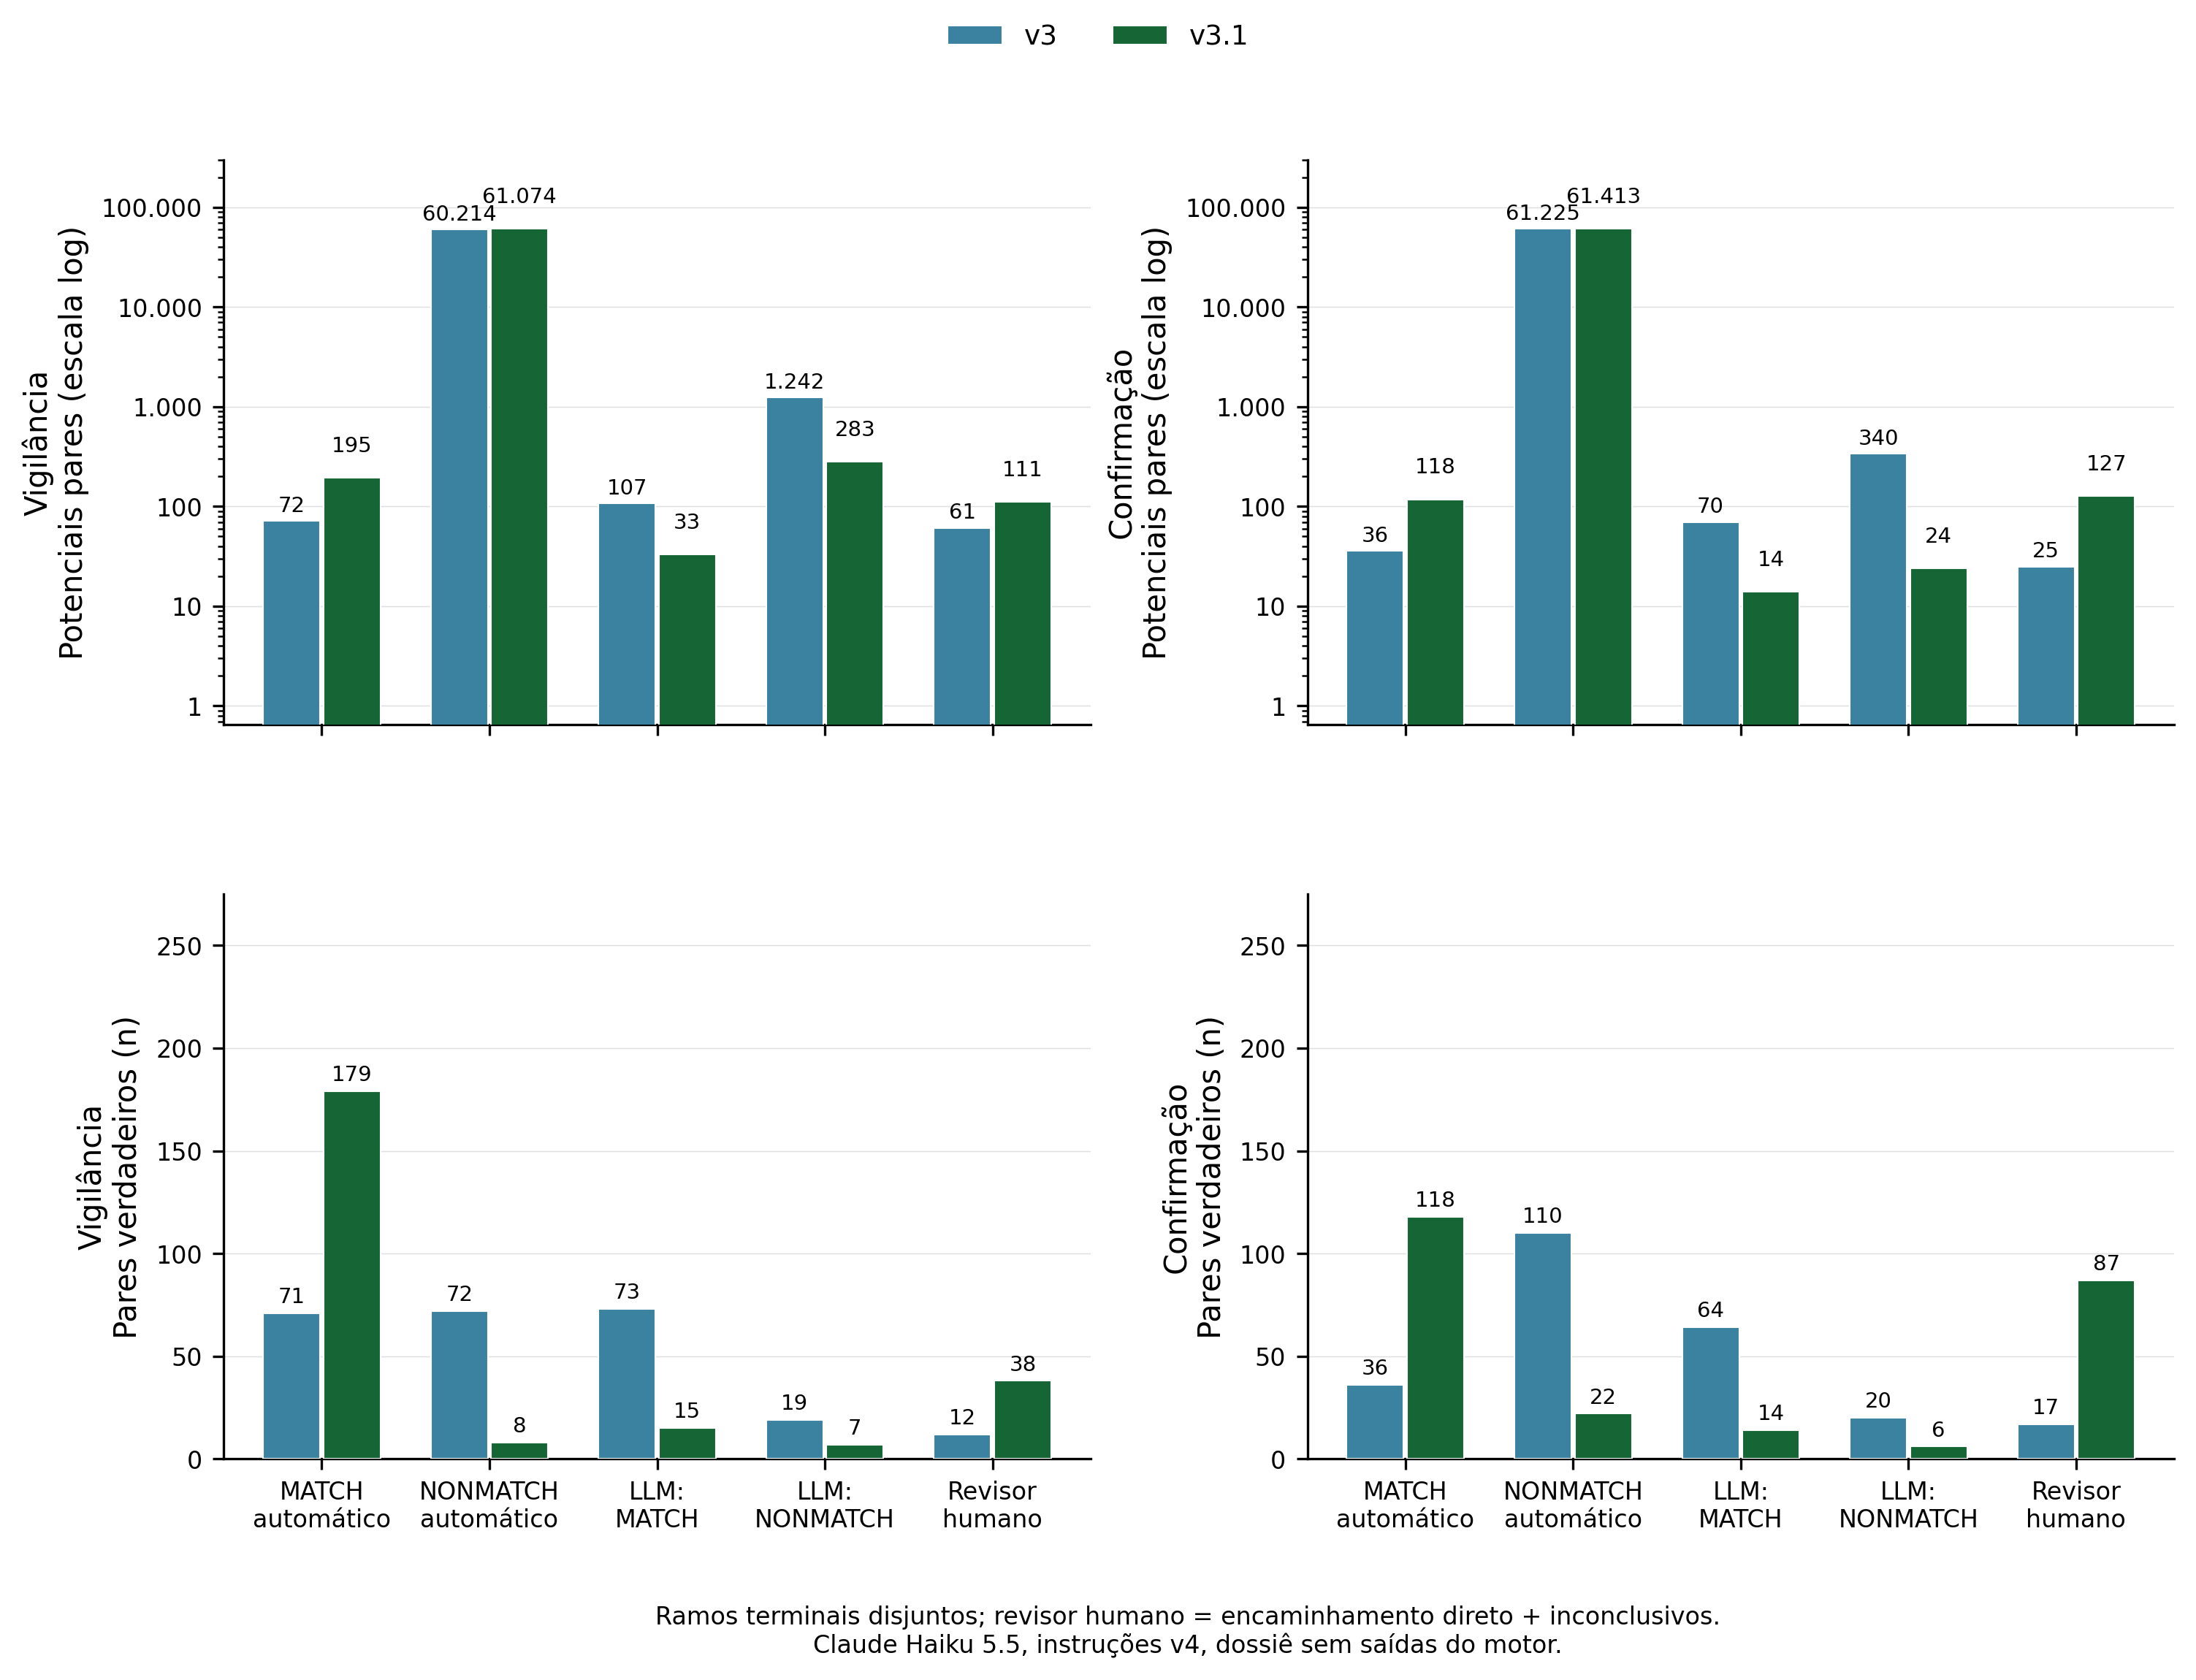
\includegraphics[width=\textwidth,height=.72\textheight,keepaspectratio]{../latex/figures/fig_cap8_cascata_v31.png}
\fonte{fig:cap8-cascata-v31; tab:cap8-cascata-v31}
\end{frame}

\begin{frame}{Backup: contagens completas da decisão final}
\small\centering
\begin{tabular}{lrrrr}
\toprule & \multicolumn{2}{c}{Vigilância} & \multicolumn{2}{c}{Confirmação} \\
& v3 & v3.1 & v3 & v3.1 \\
\midrule VP automáticos & 144 & 194 & 100 & 132 \\
FP automáticos & 35 & 34 & 6 & 0 \\
Vínculos perdidos & 91 & 15 & 130 & 28 \\
Vínculos ao humano & 12 & 38 & 17 & 87 \\
Pares ao humano & 61 & 111 & 25 & 127 \\
Pares ao LLM & 1.410 & 347 & 435 & 44 \\
\bottomrule
\end{tabular}
\medskip\par VP automáticos incluem vínculos aceitos pelo LLM.\par
Vínculos ao humano continuam no denominador da sensibilidade automática.
\fonte{tab:cap8-cascata-v31}
\end{frame}

\begin{frame}{Backup: desempenho OOF por faixa da nota}
\small\centering
\begin{tabular}{lrrrrrrr}
\toprule Faixa & Pares & Vínculos & AUC & AP & VP & FP & FN \\
\midrule $<5$ & 39.981 & 3 & n.d. & n.d. & 0 & 2 & 3 \\
$[5,6)$ & 14.263 & 17 & 1,000 & 0,721 & 12 & 7 & 5 \\
$[6,7)$ & 6.175 & 57 & 0,984 & 0,855 & 45 & 1 & 12 \\
$[7,8)$ & 1.080 & 43 & 0,995 & 0,922 & 33 & 4 & 10 \\
$[8,9)$ & 102 & 34 & 0,913 & 0,873 & 29 & 16 & 5 \\
$\geq9$ & 95 & 93 & n.d. & n.d. & 89 & 2 & 4 \\
\midrule Área cinza & 21.620 & 151 & 0,995 & 0,862 & 119 & 28 & 32 \\
\bottomrule
\end{tabular}
\medskip\par Contagens a $p\geq0,5$, fixado antes da análise. Não é a política v3.1. AUC e AP omitidas quando a classe minoritária tem menos de cinco casos.
\fonte{tab:e4-desempenho-faixas-oof}
\end{frame}

\begin{frame}{Backup: QW1 não é o fluxo Modal}
\centering
\begin{tabular}{lrr}
\toprule Modelo & $F_1$ na validação cruzada & $F_1$ no teste \\
\midrule XGBoost & $0,924\pm0,030$ & 0,920 \\
Random Forest & $0,913\pm0,029$ & 0,855 \\
MLP (64, 32) & $0,882\pm0,037$ & 0,859 \\
MLP (128, 64) & $0,872\pm0,038$ & 0,844 \\
TabNet & $0,821\pm0,055$ & 0,610 \\
\bottomrule
\end{tabular}
\medskip\par Validação $5\times5$ no treinamento e teste interno de 30\%.\par
Vazamento de alvo e partição por linha limitam a inferência. Não é validação externa nem prova de falha geral de redes neurais.
\fonte{tab:qw1-deep-learning; estudo2\_classificadores.tex, limitações}
\end{frame}

\begin{frame}{Backup: ablação por categoria, resultados exploratórios}
\small\centering
\begin{tabular}{lrr}
\toprule Categoria & $F_1$, RF & $F_1$, fluxo Modal \\
\midrule Nota $\geq8$ (referência original) & 0,610 & 0,610 \\
Somente regras (referência original) & 0,842 & 0,842 \\
Somente ML & 0,931 & 0,943 \\
Híbrido AND & 0,912 & 0,442 \\
Híbrido OR & 0,921 & 0,943 \\
ML seguido de regras & 0,853 & 0,000 \\
Regras seguidas de ML & 0,912 & 0,442 \\
Consenso ML & 0,928 & 0,943 \\
Consenso e regras & 0,896 & 0,150 \\
\bottomrule
\end{tabular}
\medskip\par Implementações de regras distintas. No fluxo Modal, nenhum vínculo do teste atinge o corte de regras 7. Limiares selecionados no teste.
\fonte{tab:ablation-best-category, redução das configurações e notas}
\end{frame}

\begin{frame}{Backup: sensibilidade ao balanceamento}
\centering
\resizebox{!}{.67\textheight}{%% Creator: Matplotlib, PGF backend
%%
%% To include the figure in your LaTeX document, write
%%   \input{<filename>.pgf}
%%
%% Make sure the required packages are loaded in your preamble
%%   \usepackage{pgf}
%%
%% Also ensure that all the required font packages are loaded; for instance,
%% the lmodern package is sometimes necessary when using math font.
%%   \usepackage{lmodern}
%%
%% Figures using additional raster images can only be included by \input if
%% they are in the same directory as the main LaTeX file. For loading figures
%% from other directories you can use the `import` package
%%   \usepackage{import}
%%
%% and then include the figures with
%%   \import{<path to file>}{<filename>.pgf}
%%
%% Matplotlib used the following preamble
%%   \def\mathdefault#1{#1}
%%   \everymath=\expandafter{\the\everymath\displaystyle}
%%   \IfFileExists{scrextend.sty}{
%%     \usepackage[fontsize=10.000000pt]{scrextend}
%%   }{
%%     \renewcommand{\normalsize}{\fontsize{10.000000}{12.000000}\selectfont}
%%     \normalsize
%%   }
%%   \usepackage[T1]{fontenc}
%%   \usepackage[utf8]{inputenc}
%%   \usepackage{lmodern}
%%   \ifdefined\pdftexversion\else  % non-pdftex case.
%%     \usepackage{fontspec}
%%     \setmainfont{DejaVuSerif.ttf}[Path=\detokenize{C:/Users/Marquinho/miniconda3/Lib/site-packages/matplotlib/mpl-data/fonts/ttf/}]
%%     \setsansfont{DejaVuSans.ttf}[Path=\detokenize{C:/Users/Marquinho/miniconda3/Lib/site-packages/matplotlib/mpl-data/fonts/ttf/}]
%%     \setmonofont{DejaVuSansMono.ttf}[Path=\detokenize{C:/Users/Marquinho/miniconda3/Lib/site-packages/matplotlib/mpl-data/fonts/ttf/}]
%%   \fi
%%   \makeatletter\@ifpackageloaded{underscore}{}{\usepackage[strings]{underscore}}\makeatother
%%
\begingroup%
\makeatletter%
\begin{pgfpicture}%
\pgfpathrectangle{\pgfpointorigin}{\pgfqpoint{7.900000in}{4.900000in}}%
\pgfusepath{use as bounding box, clip}%
\begin{pgfscope}%
\pgfsetbuttcap%
\pgfsetmiterjoin%
\definecolor{currentfill}{rgb}{1.000000,1.000000,1.000000}%
\pgfsetfillcolor{currentfill}%
\pgfsetlinewidth{0.000000pt}%
\definecolor{currentstroke}{rgb}{1.000000,1.000000,1.000000}%
\pgfsetstrokecolor{currentstroke}%
\pgfsetdash{}{0pt}%
\pgfpathmoveto{\pgfqpoint{0.000000in}{0.000000in}}%
\pgfpathlineto{\pgfqpoint{7.900000in}{0.000000in}}%
\pgfpathlineto{\pgfqpoint{7.900000in}{4.900000in}}%
\pgfpathlineto{\pgfqpoint{0.000000in}{4.900000in}}%
\pgfpathlineto{\pgfqpoint{0.000000in}{0.000000in}}%
\pgfpathclose%
\pgfusepath{fill}%
\end{pgfscope}%
\begin{pgfscope}%
\pgfsetbuttcap%
\pgfsetmiterjoin%
\definecolor{currentfill}{rgb}{1.000000,1.000000,1.000000}%
\pgfsetfillcolor{currentfill}%
\pgfsetlinewidth{0.000000pt}%
\definecolor{currentstroke}{rgb}{0.000000,0.000000,0.000000}%
\pgfsetstrokecolor{currentstroke}%
\pgfsetstrokeopacity{0.000000}%
\pgfsetdash{}{0pt}%
\pgfpathmoveto{\pgfqpoint{1.759966in}{0.514350in}}%
\pgfpathlineto{\pgfqpoint{7.641821in}{0.514350in}}%
\pgfpathlineto{\pgfqpoint{7.641821in}{4.602083in}}%
\pgfpathlineto{\pgfqpoint{1.759966in}{4.602083in}}%
\pgfpathlineto{\pgfqpoint{1.759966in}{0.514350in}}%
\pgfpathclose%
\pgfusepath{fill}%
\end{pgfscope}%
\begin{pgfscope}%
\pgfpathrectangle{\pgfqpoint{1.759966in}{0.514350in}}{\pgfqpoint{5.881855in}{4.087734in}}%
\pgfusepath{clip}%
\pgfsetbuttcap%
\pgfsetmiterjoin%
\definecolor{currentfill}{rgb}{0.301961,0.686275,0.290196}%
\pgfsetfillcolor{currentfill}%
\pgfsetfillopacity{0.850000}%
\pgfsetlinewidth{1.003750pt}%
\definecolor{currentstroke}{rgb}{1.000000,1.000000,1.000000}%
\pgfsetstrokecolor{currentstroke}%
\pgfsetstrokeopacity{0.850000}%
\pgfsetdash{}{0pt}%
\pgfpathmoveto{\pgfqpoint{-20.296989in}{0.700156in}}%
\pgfpathlineto{\pgfqpoint{5.590736in}{0.700156in}}%
\pgfpathlineto{\pgfqpoint{5.590736in}{1.037985in}}%
\pgfpathlineto{\pgfqpoint{-20.296989in}{1.037985in}}%
\pgfpathlineto{\pgfqpoint{-20.296989in}{0.700156in}}%
\pgfpathclose%
\pgfusepath{stroke,fill}%
\end{pgfscope}%
\begin{pgfscope}%
\pgfpathrectangle{\pgfqpoint{1.759966in}{0.514350in}}{\pgfqpoint{5.881855in}{4.087734in}}%
\pgfusepath{clip}%
\pgfsetbuttcap%
\pgfsetmiterjoin%
\definecolor{currentfill}{rgb}{0.301961,0.686275,0.290196}%
\pgfsetfillcolor{currentfill}%
\pgfsetfillopacity{0.850000}%
\pgfsetlinewidth{1.003750pt}%
\definecolor{currentstroke}{rgb}{1.000000,1.000000,1.000000}%
\pgfsetstrokecolor{currentstroke}%
\pgfsetstrokeopacity{0.850000}%
\pgfsetdash{}{0pt}%
\pgfpathmoveto{\pgfqpoint{-20.296989in}{1.122442in}}%
\pgfpathlineto{\pgfqpoint{6.097373in}{1.122442in}}%
\pgfpathlineto{\pgfqpoint{6.097373in}{1.460272in}}%
\pgfpathlineto{\pgfqpoint{-20.296989in}{1.460272in}}%
\pgfpathlineto{\pgfqpoint{-20.296989in}{1.122442in}}%
\pgfpathclose%
\pgfusepath{stroke,fill}%
\end{pgfscope}%
\begin{pgfscope}%
\pgfpathrectangle{\pgfqpoint{1.759966in}{0.514350in}}{\pgfqpoint{5.881855in}{4.087734in}}%
\pgfusepath{clip}%
\pgfsetbuttcap%
\pgfsetmiterjoin%
\definecolor{currentfill}{rgb}{0.301961,0.686275,0.290196}%
\pgfsetfillcolor{currentfill}%
\pgfsetfillopacity{0.850000}%
\pgfsetlinewidth{1.003750pt}%
\definecolor{currentstroke}{rgb}{1.000000,1.000000,1.000000}%
\pgfsetstrokecolor{currentstroke}%
\pgfsetstrokeopacity{0.850000}%
\pgfsetdash{}{0pt}%
\pgfpathmoveto{\pgfqpoint{-20.296989in}{1.544729in}}%
\pgfpathlineto{\pgfqpoint{6.121734in}{1.544729in}}%
\pgfpathlineto{\pgfqpoint{6.121734in}{1.882558in}}%
\pgfpathlineto{\pgfqpoint{-20.296989in}{1.882558in}}%
\pgfpathlineto{\pgfqpoint{-20.296989in}{1.544729in}}%
\pgfpathclose%
\pgfusepath{stroke,fill}%
\end{pgfscope}%
\begin{pgfscope}%
\pgfpathrectangle{\pgfqpoint{1.759966in}{0.514350in}}{\pgfqpoint{5.881855in}{4.087734in}}%
\pgfusepath{clip}%
\pgfsetbuttcap%
\pgfsetmiterjoin%
\definecolor{currentfill}{rgb}{0.301961,0.686275,0.290196}%
\pgfsetfillcolor{currentfill}%
\pgfsetfillopacity{0.850000}%
\pgfsetlinewidth{1.003750pt}%
\definecolor{currentstroke}{rgb}{1.000000,1.000000,1.000000}%
\pgfsetstrokecolor{currentstroke}%
\pgfsetstrokeopacity{0.850000}%
\pgfsetdash{}{0pt}%
\pgfpathmoveto{\pgfqpoint{-20.296989in}{1.967015in}}%
\pgfpathlineto{\pgfqpoint{6.304279in}{1.967015in}}%
\pgfpathlineto{\pgfqpoint{6.304279in}{2.304845in}}%
\pgfpathlineto{\pgfqpoint{-20.296989in}{2.304845in}}%
\pgfpathlineto{\pgfqpoint{-20.296989in}{1.967015in}}%
\pgfpathclose%
\pgfusepath{stroke,fill}%
\end{pgfscope}%
\begin{pgfscope}%
\pgfpathrectangle{\pgfqpoint{1.759966in}{0.514350in}}{\pgfqpoint{5.881855in}{4.087734in}}%
\pgfusepath{clip}%
\pgfsetbuttcap%
\pgfsetmiterjoin%
\definecolor{currentfill}{rgb}{0.301961,0.686275,0.290196}%
\pgfsetfillcolor{currentfill}%
\pgfsetfillopacity{0.850000}%
\pgfsetlinewidth{1.003750pt}%
\definecolor{currentstroke}{rgb}{1.000000,1.000000,1.000000}%
\pgfsetstrokecolor{currentstroke}%
\pgfsetstrokeopacity{0.850000}%
\pgfsetdash{}{0pt}%
\pgfpathmoveto{\pgfqpoint{-20.296989in}{2.389302in}}%
\pgfpathlineto{\pgfqpoint{6.323273in}{2.389302in}}%
\pgfpathlineto{\pgfqpoint{6.323273in}{2.727131in}}%
\pgfpathlineto{\pgfqpoint{-20.296989in}{2.727131in}}%
\pgfpathlineto{\pgfqpoint{-20.296989in}{2.389302in}}%
\pgfpathclose%
\pgfusepath{stroke,fill}%
\end{pgfscope}%
\begin{pgfscope}%
\pgfpathrectangle{\pgfqpoint{1.759966in}{0.514350in}}{\pgfqpoint{5.881855in}{4.087734in}}%
\pgfusepath{clip}%
\pgfsetbuttcap%
\pgfsetmiterjoin%
\definecolor{currentfill}{rgb}{0.301961,0.686275,0.290196}%
\pgfsetfillcolor{currentfill}%
\pgfsetfillopacity{0.850000}%
\pgfsetlinewidth{1.003750pt}%
\definecolor{currentstroke}{rgb}{1.000000,1.000000,1.000000}%
\pgfsetstrokecolor{currentstroke}%
\pgfsetstrokeopacity{0.850000}%
\pgfsetdash{}{0pt}%
\pgfpathmoveto{\pgfqpoint{-20.296989in}{2.811588in}}%
\pgfpathlineto{\pgfqpoint{6.356691in}{2.811588in}}%
\pgfpathlineto{\pgfqpoint{6.356691in}{3.149418in}}%
\pgfpathlineto{\pgfqpoint{-20.296989in}{3.149418in}}%
\pgfpathlineto{\pgfqpoint{-20.296989in}{2.811588in}}%
\pgfpathclose%
\pgfusepath{stroke,fill}%
\end{pgfscope}%
\begin{pgfscope}%
\pgfpathrectangle{\pgfqpoint{1.759966in}{0.514350in}}{\pgfqpoint{5.881855in}{4.087734in}}%
\pgfusepath{clip}%
\pgfsetbuttcap%
\pgfsetmiterjoin%
\definecolor{currentfill}{rgb}{0.301961,0.686275,0.290196}%
\pgfsetfillcolor{currentfill}%
\pgfsetfillopacity{0.850000}%
\pgfsetlinewidth{1.003750pt}%
\definecolor{currentstroke}{rgb}{1.000000,1.000000,1.000000}%
\pgfsetstrokecolor{currentstroke}%
\pgfsetstrokeopacity{0.850000}%
\pgfsetdash{}{0pt}%
\pgfpathmoveto{\pgfqpoint{-20.296989in}{3.233875in}}%
\pgfpathlineto{\pgfqpoint{6.466851in}{3.233875in}}%
\pgfpathlineto{\pgfqpoint{6.466851in}{3.571704in}}%
\pgfpathlineto{\pgfqpoint{-20.296989in}{3.571704in}}%
\pgfpathlineto{\pgfqpoint{-20.296989in}{3.233875in}}%
\pgfpathclose%
\pgfusepath{stroke,fill}%
\end{pgfscope}%
\begin{pgfscope}%
\pgfpathrectangle{\pgfqpoint{1.759966in}{0.514350in}}{\pgfqpoint{5.881855in}{4.087734in}}%
\pgfusepath{clip}%
\pgfsetbuttcap%
\pgfsetmiterjoin%
\definecolor{currentfill}{rgb}{0.301961,0.686275,0.290196}%
\pgfsetfillcolor{currentfill}%
\pgfsetfillopacity{0.850000}%
\pgfsetlinewidth{1.003750pt}%
\definecolor{currentstroke}{rgb}{1.000000,1.000000,1.000000}%
\pgfsetstrokecolor{currentstroke}%
\pgfsetstrokeopacity{0.850000}%
\pgfsetdash{}{0pt}%
\pgfpathmoveto{\pgfqpoint{-20.296989in}{3.656162in}}%
\pgfpathlineto{\pgfqpoint{6.628909in}{3.656162in}}%
\pgfpathlineto{\pgfqpoint{6.628909in}{3.993991in}}%
\pgfpathlineto{\pgfqpoint{-20.296989in}{3.993991in}}%
\pgfpathlineto{\pgfqpoint{-20.296989in}{3.656162in}}%
\pgfpathclose%
\pgfusepath{stroke,fill}%
\end{pgfscope}%
\begin{pgfscope}%
\pgfpathrectangle{\pgfqpoint{1.759966in}{0.514350in}}{\pgfqpoint{5.881855in}{4.087734in}}%
\pgfusepath{clip}%
\pgfsetbuttcap%
\pgfsetmiterjoin%
\definecolor{currentfill}{rgb}{0.301961,0.686275,0.290196}%
\pgfsetfillcolor{currentfill}%
\pgfsetfillopacity{0.850000}%
\pgfsetlinewidth{1.003750pt}%
\definecolor{currentstroke}{rgb}{1.000000,1.000000,1.000000}%
\pgfsetstrokecolor{currentstroke}%
\pgfsetstrokeopacity{0.850000}%
\pgfsetdash{}{0pt}%
\pgfpathmoveto{\pgfqpoint{-20.296989in}{4.078448in}}%
\pgfpathlineto{\pgfqpoint{6.687282in}{4.078448in}}%
\pgfpathlineto{\pgfqpoint{6.687282in}{4.416277in}}%
\pgfpathlineto{\pgfqpoint{-20.296989in}{4.416277in}}%
\pgfpathlineto{\pgfqpoint{-20.296989in}{4.078448in}}%
\pgfpathclose%
\pgfusepath{stroke,fill}%
\end{pgfscope}%
\begin{pgfscope}%
\pgfsetbuttcap%
\pgfsetroundjoin%
\definecolor{currentfill}{rgb}{0.000000,0.000000,0.000000}%
\pgfsetfillcolor{currentfill}%
\pgfsetlinewidth{0.803000pt}%
\definecolor{currentstroke}{rgb}{0.000000,0.000000,0.000000}%
\pgfsetstrokecolor{currentstroke}%
\pgfsetdash{}{0pt}%
\pgfsys@defobject{currentmarker}{\pgfqpoint{0.000000in}{-0.048611in}}{\pgfqpoint{0.000000in}{0.000000in}}{%
\pgfpathmoveto{\pgfqpoint{0.000000in}{0.000000in}}%
\pgfpathlineto{\pgfqpoint{0.000000in}{-0.048611in}}%
\pgfusepath{stroke,fill}%
}%
\begin{pgfscope}%
\pgfsys@transformshift{1.759966in}{0.514350in}%
\pgfsys@useobject{currentmarker}{}%
\end{pgfscope}%
\end{pgfscope}%
\begin{pgfscope}%
\definecolor{textcolor}{rgb}{0.000000,0.000000,0.000000}%
\pgfsetstrokecolor{textcolor}%
\pgfsetfillcolor{textcolor}%
\pgftext[x=1.759966in,y=0.417127in,,top]{\color{textcolor}{\rmfamily\fontsize{10.000000}{12.000000}\selectfont\catcode`\^=\active\def^{\ifmmode\sp\else\^{}\fi}\catcode`\%=\active\def%{\%}0.750}}%
\end{pgfscope}%
\begin{pgfscope}%
\pgfsetbuttcap%
\pgfsetroundjoin%
\definecolor{currentfill}{rgb}{0.000000,0.000000,0.000000}%
\pgfsetfillcolor{currentfill}%
\pgfsetlinewidth{0.803000pt}%
\definecolor{currentstroke}{rgb}{0.000000,0.000000,0.000000}%
\pgfsetstrokecolor{currentstroke}%
\pgfsetdash{}{0pt}%
\pgfsys@defobject{currentmarker}{\pgfqpoint{0.000000in}{-0.048611in}}{\pgfqpoint{0.000000in}{0.000000in}}{%
\pgfpathmoveto{\pgfqpoint{0.000000in}{0.000000in}}%
\pgfpathlineto{\pgfqpoint{0.000000in}{-0.048611in}}%
\pgfusepath{stroke,fill}%
}%
\begin{pgfscope}%
\pgfsys@transformshift{2.495198in}{0.514350in}%
\pgfsys@useobject{currentmarker}{}%
\end{pgfscope}%
\end{pgfscope}%
\begin{pgfscope}%
\definecolor{textcolor}{rgb}{0.000000,0.000000,0.000000}%
\pgfsetstrokecolor{textcolor}%
\pgfsetfillcolor{textcolor}%
\pgftext[x=2.495198in,y=0.417127in,,top]{\color{textcolor}{\rmfamily\fontsize{10.000000}{12.000000}\selectfont\catcode`\^=\active\def^{\ifmmode\sp\else\^{}\fi}\catcode`\%=\active\def%{\%}0.775}}%
\end{pgfscope}%
\begin{pgfscope}%
\pgfsetbuttcap%
\pgfsetroundjoin%
\definecolor{currentfill}{rgb}{0.000000,0.000000,0.000000}%
\pgfsetfillcolor{currentfill}%
\pgfsetlinewidth{0.803000pt}%
\definecolor{currentstroke}{rgb}{0.000000,0.000000,0.000000}%
\pgfsetstrokecolor{currentstroke}%
\pgfsetdash{}{0pt}%
\pgfsys@defobject{currentmarker}{\pgfqpoint{0.000000in}{-0.048611in}}{\pgfqpoint{0.000000in}{0.000000in}}{%
\pgfpathmoveto{\pgfqpoint{0.000000in}{0.000000in}}%
\pgfpathlineto{\pgfqpoint{0.000000in}{-0.048611in}}%
\pgfusepath{stroke,fill}%
}%
\begin{pgfscope}%
\pgfsys@transformshift{3.230430in}{0.514350in}%
\pgfsys@useobject{currentmarker}{}%
\end{pgfscope}%
\end{pgfscope}%
\begin{pgfscope}%
\definecolor{textcolor}{rgb}{0.000000,0.000000,0.000000}%
\pgfsetstrokecolor{textcolor}%
\pgfsetfillcolor{textcolor}%
\pgftext[x=3.230430in,y=0.417127in,,top]{\color{textcolor}{\rmfamily\fontsize{10.000000}{12.000000}\selectfont\catcode`\^=\active\def^{\ifmmode\sp\else\^{}\fi}\catcode`\%=\active\def%{\%}0.800}}%
\end{pgfscope}%
\begin{pgfscope}%
\pgfsetbuttcap%
\pgfsetroundjoin%
\definecolor{currentfill}{rgb}{0.000000,0.000000,0.000000}%
\pgfsetfillcolor{currentfill}%
\pgfsetlinewidth{0.803000pt}%
\definecolor{currentstroke}{rgb}{0.000000,0.000000,0.000000}%
\pgfsetstrokecolor{currentstroke}%
\pgfsetdash{}{0pt}%
\pgfsys@defobject{currentmarker}{\pgfqpoint{0.000000in}{-0.048611in}}{\pgfqpoint{0.000000in}{0.000000in}}{%
\pgfpathmoveto{\pgfqpoint{0.000000in}{0.000000in}}%
\pgfpathlineto{\pgfqpoint{0.000000in}{-0.048611in}}%
\pgfusepath{stroke,fill}%
}%
\begin{pgfscope}%
\pgfsys@transformshift{3.965662in}{0.514350in}%
\pgfsys@useobject{currentmarker}{}%
\end{pgfscope}%
\end{pgfscope}%
\begin{pgfscope}%
\definecolor{textcolor}{rgb}{0.000000,0.000000,0.000000}%
\pgfsetstrokecolor{textcolor}%
\pgfsetfillcolor{textcolor}%
\pgftext[x=3.965662in,y=0.417127in,,top]{\color{textcolor}{\rmfamily\fontsize{10.000000}{12.000000}\selectfont\catcode`\^=\active\def^{\ifmmode\sp\else\^{}\fi}\catcode`\%=\active\def%{\%}0.825}}%
\end{pgfscope}%
\begin{pgfscope}%
\pgfsetbuttcap%
\pgfsetroundjoin%
\definecolor{currentfill}{rgb}{0.000000,0.000000,0.000000}%
\pgfsetfillcolor{currentfill}%
\pgfsetlinewidth{0.803000pt}%
\definecolor{currentstroke}{rgb}{0.000000,0.000000,0.000000}%
\pgfsetstrokecolor{currentstroke}%
\pgfsetdash{}{0pt}%
\pgfsys@defobject{currentmarker}{\pgfqpoint{0.000000in}{-0.048611in}}{\pgfqpoint{0.000000in}{0.000000in}}{%
\pgfpathmoveto{\pgfqpoint{0.000000in}{0.000000in}}%
\pgfpathlineto{\pgfqpoint{0.000000in}{-0.048611in}}%
\pgfusepath{stroke,fill}%
}%
\begin{pgfscope}%
\pgfsys@transformshift{4.700894in}{0.514350in}%
\pgfsys@useobject{currentmarker}{}%
\end{pgfscope}%
\end{pgfscope}%
\begin{pgfscope}%
\definecolor{textcolor}{rgb}{0.000000,0.000000,0.000000}%
\pgfsetstrokecolor{textcolor}%
\pgfsetfillcolor{textcolor}%
\pgftext[x=4.700894in,y=0.417127in,,top]{\color{textcolor}{\rmfamily\fontsize{10.000000}{12.000000}\selectfont\catcode`\^=\active\def^{\ifmmode\sp\else\^{}\fi}\catcode`\%=\active\def%{\%}0.850}}%
\end{pgfscope}%
\begin{pgfscope}%
\pgfsetbuttcap%
\pgfsetroundjoin%
\definecolor{currentfill}{rgb}{0.000000,0.000000,0.000000}%
\pgfsetfillcolor{currentfill}%
\pgfsetlinewidth{0.803000pt}%
\definecolor{currentstroke}{rgb}{0.000000,0.000000,0.000000}%
\pgfsetstrokecolor{currentstroke}%
\pgfsetdash{}{0pt}%
\pgfsys@defobject{currentmarker}{\pgfqpoint{0.000000in}{-0.048611in}}{\pgfqpoint{0.000000in}{0.000000in}}{%
\pgfpathmoveto{\pgfqpoint{0.000000in}{0.000000in}}%
\pgfpathlineto{\pgfqpoint{0.000000in}{-0.048611in}}%
\pgfusepath{stroke,fill}%
}%
\begin{pgfscope}%
\pgfsys@transformshift{5.436126in}{0.514350in}%
\pgfsys@useobject{currentmarker}{}%
\end{pgfscope}%
\end{pgfscope}%
\begin{pgfscope}%
\definecolor{textcolor}{rgb}{0.000000,0.000000,0.000000}%
\pgfsetstrokecolor{textcolor}%
\pgfsetfillcolor{textcolor}%
\pgftext[x=5.436126in,y=0.417127in,,top]{\color{textcolor}{\rmfamily\fontsize{10.000000}{12.000000}\selectfont\catcode`\^=\active\def^{\ifmmode\sp\else\^{}\fi}\catcode`\%=\active\def%{\%}0.875}}%
\end{pgfscope}%
\begin{pgfscope}%
\pgfsetbuttcap%
\pgfsetroundjoin%
\definecolor{currentfill}{rgb}{0.000000,0.000000,0.000000}%
\pgfsetfillcolor{currentfill}%
\pgfsetlinewidth{0.803000pt}%
\definecolor{currentstroke}{rgb}{0.000000,0.000000,0.000000}%
\pgfsetstrokecolor{currentstroke}%
\pgfsetdash{}{0pt}%
\pgfsys@defobject{currentmarker}{\pgfqpoint{0.000000in}{-0.048611in}}{\pgfqpoint{0.000000in}{0.000000in}}{%
\pgfpathmoveto{\pgfqpoint{0.000000in}{0.000000in}}%
\pgfpathlineto{\pgfqpoint{0.000000in}{-0.048611in}}%
\pgfusepath{stroke,fill}%
}%
\begin{pgfscope}%
\pgfsys@transformshift{6.171357in}{0.514350in}%
\pgfsys@useobject{currentmarker}{}%
\end{pgfscope}%
\end{pgfscope}%
\begin{pgfscope}%
\definecolor{textcolor}{rgb}{0.000000,0.000000,0.000000}%
\pgfsetstrokecolor{textcolor}%
\pgfsetfillcolor{textcolor}%
\pgftext[x=6.171357in,y=0.417127in,,top]{\color{textcolor}{\rmfamily\fontsize{10.000000}{12.000000}\selectfont\catcode`\^=\active\def^{\ifmmode\sp\else\^{}\fi}\catcode`\%=\active\def%{\%}0.900}}%
\end{pgfscope}%
\begin{pgfscope}%
\pgfsetbuttcap%
\pgfsetroundjoin%
\definecolor{currentfill}{rgb}{0.000000,0.000000,0.000000}%
\pgfsetfillcolor{currentfill}%
\pgfsetlinewidth{0.803000pt}%
\definecolor{currentstroke}{rgb}{0.000000,0.000000,0.000000}%
\pgfsetstrokecolor{currentstroke}%
\pgfsetdash{}{0pt}%
\pgfsys@defobject{currentmarker}{\pgfqpoint{0.000000in}{-0.048611in}}{\pgfqpoint{0.000000in}{0.000000in}}{%
\pgfpathmoveto{\pgfqpoint{0.000000in}{0.000000in}}%
\pgfpathlineto{\pgfqpoint{0.000000in}{-0.048611in}}%
\pgfusepath{stroke,fill}%
}%
\begin{pgfscope}%
\pgfsys@transformshift{6.906589in}{0.514350in}%
\pgfsys@useobject{currentmarker}{}%
\end{pgfscope}%
\end{pgfscope}%
\begin{pgfscope}%
\definecolor{textcolor}{rgb}{0.000000,0.000000,0.000000}%
\pgfsetstrokecolor{textcolor}%
\pgfsetfillcolor{textcolor}%
\pgftext[x=6.906589in,y=0.417127in,,top]{\color{textcolor}{\rmfamily\fontsize{10.000000}{12.000000}\selectfont\catcode`\^=\active\def^{\ifmmode\sp\else\^{}\fi}\catcode`\%=\active\def%{\%}0.925}}%
\end{pgfscope}%
\begin{pgfscope}%
\pgfsetbuttcap%
\pgfsetroundjoin%
\definecolor{currentfill}{rgb}{0.000000,0.000000,0.000000}%
\pgfsetfillcolor{currentfill}%
\pgfsetlinewidth{0.803000pt}%
\definecolor{currentstroke}{rgb}{0.000000,0.000000,0.000000}%
\pgfsetstrokecolor{currentstroke}%
\pgfsetdash{}{0pt}%
\pgfsys@defobject{currentmarker}{\pgfqpoint{0.000000in}{-0.048611in}}{\pgfqpoint{0.000000in}{0.000000in}}{%
\pgfpathmoveto{\pgfqpoint{0.000000in}{0.000000in}}%
\pgfpathlineto{\pgfqpoint{0.000000in}{-0.048611in}}%
\pgfusepath{stroke,fill}%
}%
\begin{pgfscope}%
\pgfsys@transformshift{7.641821in}{0.514350in}%
\pgfsys@useobject{currentmarker}{}%
\end{pgfscope}%
\end{pgfscope}%
\begin{pgfscope}%
\definecolor{textcolor}{rgb}{0.000000,0.000000,0.000000}%
\pgfsetstrokecolor{textcolor}%
\pgfsetfillcolor{textcolor}%
\pgftext[x=7.641821in,y=0.417127in,,top]{\color{textcolor}{\rmfamily\fontsize{10.000000}{12.000000}\selectfont\catcode`\^=\active\def^{\ifmmode\sp\else\^{}\fi}\catcode`\%=\active\def%{\%}0.950}}%
\end{pgfscope}%
\begin{pgfscope}%
\definecolor{textcolor}{rgb}{0.000000,0.000000,0.000000}%
\pgfsetstrokecolor{textcolor}%
\pgfsetfillcolor{textcolor}%
\pgftext[x=4.700894in,y=0.238889in,,top]{\color{textcolor}{\rmfamily\fontsize{10.000000}{12.000000}\selectfont\catcode`\^=\active\def^{\ifmmode\sp\else\^{}\fi}\catcode`\%=\active\def%{\%}F1-score (média ± desvio, 5-fold CV)}}%
\end{pgfscope}%
\begin{pgfscope}%
\pgfsetbuttcap%
\pgfsetroundjoin%
\definecolor{currentfill}{rgb}{0.000000,0.000000,0.000000}%
\pgfsetfillcolor{currentfill}%
\pgfsetlinewidth{0.803000pt}%
\definecolor{currentstroke}{rgb}{0.000000,0.000000,0.000000}%
\pgfsetstrokecolor{currentstroke}%
\pgfsetdash{}{0pt}%
\pgfsys@defobject{currentmarker}{\pgfqpoint{-0.048611in}{0.000000in}}{\pgfqpoint{-0.000000in}{0.000000in}}{%
\pgfpathmoveto{\pgfqpoint{-0.000000in}{0.000000in}}%
\pgfpathlineto{\pgfqpoint{-0.048611in}{0.000000in}}%
\pgfusepath{stroke,fill}%
}%
\begin{pgfscope}%
\pgfsys@transformshift{1.759966in}{0.869070in}%
\pgfsys@useobject{currentmarker}{}%
\end{pgfscope}%
\end{pgfscope}%
\begin{pgfscope}%
\definecolor{textcolor}{rgb}{0.000000,0.000000,0.000000}%
\pgfsetstrokecolor{textcolor}%
\pgfsetfillcolor{textcolor}%
\pgftext[x=0.369360in, y=0.826015in, left, base]{\color{textcolor}{\rmfamily\fontsize{9.000000}{10.800000}\selectfont\catcode`\^=\active\def^{\ifmmode\sp\else\^{}\fi}\catcode`\%=\active\def%{\%}Class weight=balanced}}%
\end{pgfscope}%
\begin{pgfscope}%
\pgfsetbuttcap%
\pgfsetroundjoin%
\definecolor{currentfill}{rgb}{0.000000,0.000000,0.000000}%
\pgfsetfillcolor{currentfill}%
\pgfsetlinewidth{0.803000pt}%
\definecolor{currentstroke}{rgb}{0.000000,0.000000,0.000000}%
\pgfsetstrokecolor{currentstroke}%
\pgfsetdash{}{0pt}%
\pgfsys@defobject{currentmarker}{\pgfqpoint{-0.048611in}{0.000000in}}{\pgfqpoint{-0.000000in}{0.000000in}}{%
\pgfpathmoveto{\pgfqpoint{-0.000000in}{0.000000in}}%
\pgfpathlineto{\pgfqpoint{-0.048611in}{0.000000in}}%
\pgfusepath{stroke,fill}%
}%
\begin{pgfscope}%
\pgfsys@transformshift{1.759966in}{1.291357in}%
\pgfsys@useobject{currentmarker}{}%
\end{pgfscope}%
\end{pgfscope}%
\begin{pgfscope}%
\definecolor{textcolor}{rgb}{0.000000,0.000000,0.000000}%
\pgfsetstrokecolor{textcolor}%
\pgfsetfillcolor{textcolor}%
\pgftext[x=0.924045in, y=1.248301in, left, base]{\color{textcolor}{\rmfamily\fontsize{9.000000}{10.800000}\selectfont\catcode`\^=\active\def^{\ifmmode\sp\else\^{}\fi}\catcode`\%=\active\def%{\%}No balancing}}%
\end{pgfscope}%
\begin{pgfscope}%
\pgfsetbuttcap%
\pgfsetroundjoin%
\definecolor{currentfill}{rgb}{0.000000,0.000000,0.000000}%
\pgfsetfillcolor{currentfill}%
\pgfsetlinewidth{0.803000pt}%
\definecolor{currentstroke}{rgb}{0.000000,0.000000,0.000000}%
\pgfsetstrokecolor{currentstroke}%
\pgfsetdash{}{0pt}%
\pgfsys@defobject{currentmarker}{\pgfqpoint{-0.048611in}{0.000000in}}{\pgfqpoint{-0.000000in}{0.000000in}}{%
\pgfpathmoveto{\pgfqpoint{-0.000000in}{0.000000in}}%
\pgfpathlineto{\pgfqpoint{-0.048611in}{0.000000in}}%
\pgfusepath{stroke,fill}%
}%
\begin{pgfscope}%
\pgfsys@transformshift{1.759966in}{1.713643in}%
\pgfsys@useobject{currentmarker}{}%
\end{pgfscope}%
\end{pgfscope}%
\begin{pgfscope}%
\definecolor{textcolor}{rgb}{0.000000,0.000000,0.000000}%
\pgfsetstrokecolor{textcolor}%
\pgfsetfillcolor{textcolor}%
\pgftext[x=0.100000in, y=1.670588in, left, base]{\color{textcolor}{\rmfamily\fontsize{9.000000}{10.800000}\selectfont\catcode`\^=\active\def^{\ifmmode\sp\else\^{}\fi}\catcode`\%=\active\def%{\%}Class weight + SMOTE 0.3}}%
\end{pgfscope}%
\begin{pgfscope}%
\pgfsetbuttcap%
\pgfsetroundjoin%
\definecolor{currentfill}{rgb}{0.000000,0.000000,0.000000}%
\pgfsetfillcolor{currentfill}%
\pgfsetlinewidth{0.803000pt}%
\definecolor{currentstroke}{rgb}{0.000000,0.000000,0.000000}%
\pgfsetstrokecolor{currentstroke}%
\pgfsetdash{}{0pt}%
\pgfsys@defobject{currentmarker}{\pgfqpoint{-0.048611in}{0.000000in}}{\pgfqpoint{-0.000000in}{0.000000in}}{%
\pgfpathmoveto{\pgfqpoint{-0.000000in}{0.000000in}}%
\pgfpathlineto{\pgfqpoint{-0.048611in}{0.000000in}}%
\pgfusepath{stroke,fill}%
}%
\begin{pgfscope}%
\pgfsys@transformshift{1.759966in}{2.135930in}%
\pgfsys@useobject{currentmarker}{}%
\end{pgfscope}%
\end{pgfscope}%
\begin{pgfscope}%
\definecolor{textcolor}{rgb}{0.000000,0.000000,0.000000}%
\pgfsetstrokecolor{textcolor}%
\pgfsetfillcolor{textcolor}%
\pgftext[x=0.986504in, y=2.092874in, left, base]{\color{textcolor}{\rmfamily\fontsize{9.000000}{10.800000}\selectfont\catcode`\^=\active\def^{\ifmmode\sp\else\^{}\fi}\catcode`\%=\active\def%{\%}SMOTE 1.0}}%
\end{pgfscope}%
\begin{pgfscope}%
\pgfsetbuttcap%
\pgfsetroundjoin%
\definecolor{currentfill}{rgb}{0.000000,0.000000,0.000000}%
\pgfsetfillcolor{currentfill}%
\pgfsetlinewidth{0.803000pt}%
\definecolor{currentstroke}{rgb}{0.000000,0.000000,0.000000}%
\pgfsetstrokecolor{currentstroke}%
\pgfsetdash{}{0pt}%
\pgfsys@defobject{currentmarker}{\pgfqpoint{-0.048611in}{0.000000in}}{\pgfqpoint{-0.000000in}{0.000000in}}{%
\pgfpathmoveto{\pgfqpoint{-0.000000in}{0.000000in}}%
\pgfpathlineto{\pgfqpoint{-0.048611in}{0.000000in}}%
\pgfusepath{stroke,fill}%
}%
\begin{pgfscope}%
\pgfsys@transformshift{1.759966in}{2.558217in}%
\pgfsys@useobject{currentmarker}{}%
\end{pgfscope}%
\end{pgfscope}%
\begin{pgfscope}%
\definecolor{textcolor}{rgb}{0.000000,0.000000,0.000000}%
\pgfsetstrokecolor{textcolor}%
\pgfsetfillcolor{textcolor}%
\pgftext[x=0.402359in, y=2.515161in, left, base]{\color{textcolor}{\rmfamily\fontsize{9.000000}{10.800000}\selectfont\catcode`\^=\active\def^{\ifmmode\sp\else\^{}\fi}\catcode`\%=\active\def%{\%}BorderlineSMOTE 0.3}}%
\end{pgfscope}%
\begin{pgfscope}%
\pgfsetbuttcap%
\pgfsetroundjoin%
\definecolor{currentfill}{rgb}{0.000000,0.000000,0.000000}%
\pgfsetfillcolor{currentfill}%
\pgfsetlinewidth{0.803000pt}%
\definecolor{currentstroke}{rgb}{0.000000,0.000000,0.000000}%
\pgfsetstrokecolor{currentstroke}%
\pgfsetdash{}{0pt}%
\pgfsys@defobject{currentmarker}{\pgfqpoint{-0.048611in}{0.000000in}}{\pgfqpoint{-0.000000in}{0.000000in}}{%
\pgfpathmoveto{\pgfqpoint{-0.000000in}{0.000000in}}%
\pgfpathlineto{\pgfqpoint{-0.048611in}{0.000000in}}%
\pgfusepath{stroke,fill}%
}%
\begin{pgfscope}%
\pgfsys@transformshift{1.759966in}{2.980503in}%
\pgfsys@useobject{currentmarker}{}%
\end{pgfscope}%
\end{pgfscope}%
\begin{pgfscope}%
\definecolor{textcolor}{rgb}{0.000000,0.000000,0.000000}%
\pgfsetstrokecolor{textcolor}%
\pgfsetfillcolor{textcolor}%
\pgftext[x=0.904497in, y=2.937448in, left, base]{\color{textcolor}{\rmfamily\fontsize{9.000000}{10.800000}\selectfont\catcode`\^=\active\def^{\ifmmode\sp\else\^{}\fi}\catcode`\%=\active\def%{\%}ADASYN 0.3}}%
\end{pgfscope}%
\begin{pgfscope}%
\pgfsetbuttcap%
\pgfsetroundjoin%
\definecolor{currentfill}{rgb}{0.000000,0.000000,0.000000}%
\pgfsetfillcolor{currentfill}%
\pgfsetlinewidth{0.803000pt}%
\definecolor{currentstroke}{rgb}{0.000000,0.000000,0.000000}%
\pgfsetstrokecolor{currentstroke}%
\pgfsetdash{}{0pt}%
\pgfsys@defobject{currentmarker}{\pgfqpoint{-0.048611in}{0.000000in}}{\pgfqpoint{-0.000000in}{0.000000in}}{%
\pgfpathmoveto{\pgfqpoint{-0.000000in}{0.000000in}}%
\pgfpathlineto{\pgfqpoint{-0.048611in}{0.000000in}}%
\pgfusepath{stroke,fill}%
}%
\begin{pgfscope}%
\pgfsys@transformshift{1.759966in}{3.402790in}%
\pgfsys@useobject{currentmarker}{}%
\end{pgfscope}%
\end{pgfscope}%
\begin{pgfscope}%
\definecolor{textcolor}{rgb}{0.000000,0.000000,0.000000}%
\pgfsetstrokecolor{textcolor}%
\pgfsetfillcolor{textcolor}%
\pgftext[x=0.986504in, y=3.359734in, left, base]{\color{textcolor}{\rmfamily\fontsize{9.000000}{10.800000}\selectfont\catcode`\^=\active\def^{\ifmmode\sp\else\^{}\fi}\catcode`\%=\active\def%{\%}SMOTE 0.5}}%
\end{pgfscope}%
\begin{pgfscope}%
\pgfsetbuttcap%
\pgfsetroundjoin%
\definecolor{currentfill}{rgb}{0.000000,0.000000,0.000000}%
\pgfsetfillcolor{currentfill}%
\pgfsetlinewidth{0.803000pt}%
\definecolor{currentstroke}{rgb}{0.000000,0.000000,0.000000}%
\pgfsetstrokecolor{currentstroke}%
\pgfsetdash{}{0pt}%
\pgfsys@defobject{currentmarker}{\pgfqpoint{-0.048611in}{0.000000in}}{\pgfqpoint{-0.000000in}{0.000000in}}{%
\pgfpathmoveto{\pgfqpoint{-0.000000in}{0.000000in}}%
\pgfpathlineto{\pgfqpoint{-0.048611in}{0.000000in}}%
\pgfusepath{stroke,fill}%
}%
\begin{pgfscope}%
\pgfsys@transformshift{1.759966in}{3.825076in}%
\pgfsys@useobject{currentmarker}{}%
\end{pgfscope}%
\end{pgfscope}%
\begin{pgfscope}%
\definecolor{textcolor}{rgb}{0.000000,0.000000,0.000000}%
\pgfsetstrokecolor{textcolor}%
\pgfsetfillcolor{textcolor}%
\pgftext[x=0.986504in, y=3.782021in, left, base]{\color{textcolor}{\rmfamily\fontsize{9.000000}{10.800000}\selectfont\catcode`\^=\active\def^{\ifmmode\sp\else\^{}\fi}\catcode`\%=\active\def%{\%}SMOTE 0.3}}%
\end{pgfscope}%
\begin{pgfscope}%
\pgfsetbuttcap%
\pgfsetroundjoin%
\definecolor{currentfill}{rgb}{0.000000,0.000000,0.000000}%
\pgfsetfillcolor{currentfill}%
\pgfsetlinewidth{0.803000pt}%
\definecolor{currentstroke}{rgb}{0.000000,0.000000,0.000000}%
\pgfsetstrokecolor{currentstroke}%
\pgfsetdash{}{0pt}%
\pgfsys@defobject{currentmarker}{\pgfqpoint{-0.048611in}{0.000000in}}{\pgfqpoint{-0.000000in}{0.000000in}}{%
\pgfpathmoveto{\pgfqpoint{-0.000000in}{0.000000in}}%
\pgfpathlineto{\pgfqpoint{-0.048611in}{0.000000in}}%
\pgfusepath{stroke,fill}%
}%
\begin{pgfscope}%
\pgfsys@transformshift{1.759966in}{4.247363in}%
\pgfsys@useobject{currentmarker}{}%
\end{pgfscope}%
\end{pgfscope}%
\begin{pgfscope}%
\definecolor{textcolor}{rgb}{0.000000,0.000000,0.000000}%
\pgfsetstrokecolor{textcolor}%
\pgfsetfillcolor{textcolor}%
\pgftext[x=0.608183in, y=4.204307in, left, base]{\color{textcolor}{\rmfamily\fontsize{9.000000}{10.800000}\selectfont\catcode`\^=\active\def^{\ifmmode\sp\else\^{}\fi}\catcode`\%=\active\def%{\%}SMOTETomek 0.3}}%
\end{pgfscope}%
\begin{pgfscope}%
\pgfpathrectangle{\pgfqpoint{1.759966in}{0.514350in}}{\pgfqpoint{5.881855in}{4.087734in}}%
\pgfusepath{clip}%
\pgfsetbuttcap%
\pgfsetroundjoin%
\pgfsetlinewidth{1.505625pt}%
\definecolor{currentstroke}{rgb}{0.000000,0.000000,0.000000}%
\pgfsetstrokecolor{currentstroke}%
\pgfsetdash{}{0pt}%
\pgfpathmoveto{\pgfqpoint{4.389587in}{0.869070in}}%
\pgfpathlineto{\pgfqpoint{6.791885in}{0.869070in}}%
\pgfusepath{stroke}%
\end{pgfscope}%
\begin{pgfscope}%
\pgfpathrectangle{\pgfqpoint{1.759966in}{0.514350in}}{\pgfqpoint{5.881855in}{4.087734in}}%
\pgfusepath{clip}%
\pgfsetbuttcap%
\pgfsetroundjoin%
\pgfsetlinewidth{1.505625pt}%
\definecolor{currentstroke}{rgb}{0.000000,0.000000,0.000000}%
\pgfsetstrokecolor{currentstroke}%
\pgfsetdash{}{0pt}%
\pgfpathmoveto{\pgfqpoint{4.898917in}{1.291357in}}%
\pgfpathlineto{\pgfqpoint{7.295829in}{1.291357in}}%
\pgfusepath{stroke}%
\end{pgfscope}%
\begin{pgfscope}%
\pgfpathrectangle{\pgfqpoint{1.759966in}{0.514350in}}{\pgfqpoint{5.881855in}{4.087734in}}%
\pgfusepath{clip}%
\pgfsetbuttcap%
\pgfsetroundjoin%
\pgfsetlinewidth{1.505625pt}%
\definecolor{currentstroke}{rgb}{0.000000,0.000000,0.000000}%
\pgfsetstrokecolor{currentstroke}%
\pgfsetdash{}{0pt}%
\pgfpathmoveto{\pgfqpoint{5.411543in}{1.713643in}}%
\pgfpathlineto{\pgfqpoint{6.831924in}{1.713643in}}%
\pgfusepath{stroke}%
\end{pgfscope}%
\begin{pgfscope}%
\pgfpathrectangle{\pgfqpoint{1.759966in}{0.514350in}}{\pgfqpoint{5.881855in}{4.087734in}}%
\pgfusepath{clip}%
\pgfsetbuttcap%
\pgfsetroundjoin%
\pgfsetlinewidth{1.505625pt}%
\definecolor{currentstroke}{rgb}{0.000000,0.000000,0.000000}%
\pgfsetstrokecolor{currentstroke}%
\pgfsetdash{}{0pt}%
\pgfpathmoveto{\pgfqpoint{5.661227in}{2.135930in}}%
\pgfpathlineto{\pgfqpoint{6.947330in}{2.135930in}}%
\pgfusepath{stroke}%
\end{pgfscope}%
\begin{pgfscope}%
\pgfpathrectangle{\pgfqpoint{1.759966in}{0.514350in}}{\pgfqpoint{5.881855in}{4.087734in}}%
\pgfusepath{clip}%
\pgfsetbuttcap%
\pgfsetroundjoin%
\pgfsetlinewidth{1.505625pt}%
\definecolor{currentstroke}{rgb}{0.000000,0.000000,0.000000}%
\pgfsetstrokecolor{currentstroke}%
\pgfsetdash{}{0pt}%
\pgfpathmoveto{\pgfqpoint{5.559944in}{2.558217in}}%
\pgfpathlineto{\pgfqpoint{7.086602in}{2.558217in}}%
\pgfusepath{stroke}%
\end{pgfscope}%
\begin{pgfscope}%
\pgfpathrectangle{\pgfqpoint{1.759966in}{0.514350in}}{\pgfqpoint{5.881855in}{4.087734in}}%
\pgfusepath{clip}%
\pgfsetbuttcap%
\pgfsetroundjoin%
\pgfsetlinewidth{1.505625pt}%
\definecolor{currentstroke}{rgb}{0.000000,0.000000,0.000000}%
\pgfsetstrokecolor{currentstroke}%
\pgfsetdash{}{0pt}%
\pgfpathmoveto{\pgfqpoint{5.743915in}{2.980503in}}%
\pgfpathlineto{\pgfqpoint{6.969468in}{2.980503in}}%
\pgfusepath{stroke}%
\end{pgfscope}%
\begin{pgfscope}%
\pgfpathrectangle{\pgfqpoint{1.759966in}{0.514350in}}{\pgfqpoint{5.881855in}{4.087734in}}%
\pgfusepath{clip}%
\pgfsetbuttcap%
\pgfsetroundjoin%
\pgfsetlinewidth{1.505625pt}%
\definecolor{currentstroke}{rgb}{0.000000,0.000000,0.000000}%
\pgfsetstrokecolor{currentstroke}%
\pgfsetdash{}{0pt}%
\pgfpathmoveto{\pgfqpoint{5.941311in}{3.402790in}}%
\pgfpathlineto{\pgfqpoint{6.992391in}{3.402790in}}%
\pgfusepath{stroke}%
\end{pgfscope}%
\begin{pgfscope}%
\pgfpathrectangle{\pgfqpoint{1.759966in}{0.514350in}}{\pgfqpoint{5.881855in}{4.087734in}}%
\pgfusepath{clip}%
\pgfsetbuttcap%
\pgfsetroundjoin%
\pgfsetlinewidth{1.505625pt}%
\definecolor{currentstroke}{rgb}{0.000000,0.000000,0.000000}%
\pgfsetstrokecolor{currentstroke}%
\pgfsetdash{}{0pt}%
\pgfpathmoveto{\pgfqpoint{5.870197in}{3.825076in}}%
\pgfpathlineto{\pgfqpoint{7.387621in}{3.825076in}}%
\pgfusepath{stroke}%
\end{pgfscope}%
\begin{pgfscope}%
\pgfpathrectangle{\pgfqpoint{1.759966in}{0.514350in}}{\pgfqpoint{5.881855in}{4.087734in}}%
\pgfusepath{clip}%
\pgfsetbuttcap%
\pgfsetroundjoin%
\pgfsetlinewidth{1.505625pt}%
\definecolor{currentstroke}{rgb}{0.000000,0.000000,0.000000}%
\pgfsetstrokecolor{currentstroke}%
\pgfsetdash{}{0pt}%
\pgfpathmoveto{\pgfqpoint{5.985640in}{4.247363in}}%
\pgfpathlineto{\pgfqpoint{7.388924in}{4.247363in}}%
\pgfusepath{stroke}%
\end{pgfscope}%
\begin{pgfscope}%
\pgfpathrectangle{\pgfqpoint{1.759966in}{0.514350in}}{\pgfqpoint{5.881855in}{4.087734in}}%
\pgfusepath{clip}%
\pgfsetbuttcap%
\pgfsetroundjoin%
\definecolor{currentfill}{rgb}{0.121569,0.466667,0.705882}%
\pgfsetfillcolor{currentfill}%
\pgfsetlinewidth{1.003750pt}%
\definecolor{currentstroke}{rgb}{0.000000,0.000000,0.000000}%
\pgfsetstrokecolor{currentstroke}%
\pgfsetdash{}{0pt}%
\pgfsys@defobject{currentmarker}{\pgfqpoint{0.000000in}{-0.041667in}}{\pgfqpoint{0.000000in}{0.041667in}}{%
\pgfpathmoveto{\pgfqpoint{0.000000in}{-0.041667in}}%
\pgfpathlineto{\pgfqpoint{0.000000in}{0.041667in}}%
\pgfusepath{stroke,fill}%
}%
\begin{pgfscope}%
\pgfsys@transformshift{4.389587in}{0.869070in}%
\pgfsys@useobject{currentmarker}{}%
\end{pgfscope}%
\begin{pgfscope}%
\pgfsys@transformshift{4.898917in}{1.291357in}%
\pgfsys@useobject{currentmarker}{}%
\end{pgfscope}%
\begin{pgfscope}%
\pgfsys@transformshift{5.411543in}{1.713643in}%
\pgfsys@useobject{currentmarker}{}%
\end{pgfscope}%
\begin{pgfscope}%
\pgfsys@transformshift{5.661227in}{2.135930in}%
\pgfsys@useobject{currentmarker}{}%
\end{pgfscope}%
\begin{pgfscope}%
\pgfsys@transformshift{5.559944in}{2.558217in}%
\pgfsys@useobject{currentmarker}{}%
\end{pgfscope}%
\begin{pgfscope}%
\pgfsys@transformshift{5.743915in}{2.980503in}%
\pgfsys@useobject{currentmarker}{}%
\end{pgfscope}%
\begin{pgfscope}%
\pgfsys@transformshift{5.941311in}{3.402790in}%
\pgfsys@useobject{currentmarker}{}%
\end{pgfscope}%
\begin{pgfscope}%
\pgfsys@transformshift{5.870197in}{3.825076in}%
\pgfsys@useobject{currentmarker}{}%
\end{pgfscope}%
\begin{pgfscope}%
\pgfsys@transformshift{5.985640in}{4.247363in}%
\pgfsys@useobject{currentmarker}{}%
\end{pgfscope}%
\end{pgfscope}%
\begin{pgfscope}%
\pgfpathrectangle{\pgfqpoint{1.759966in}{0.514350in}}{\pgfqpoint{5.881855in}{4.087734in}}%
\pgfusepath{clip}%
\pgfsetbuttcap%
\pgfsetroundjoin%
\definecolor{currentfill}{rgb}{0.121569,0.466667,0.705882}%
\pgfsetfillcolor{currentfill}%
\pgfsetlinewidth{1.003750pt}%
\definecolor{currentstroke}{rgb}{0.000000,0.000000,0.000000}%
\pgfsetstrokecolor{currentstroke}%
\pgfsetdash{}{0pt}%
\pgfsys@defobject{currentmarker}{\pgfqpoint{0.000000in}{-0.041667in}}{\pgfqpoint{0.000000in}{0.041667in}}{%
\pgfpathmoveto{\pgfqpoint{0.000000in}{-0.041667in}}%
\pgfpathlineto{\pgfqpoint{0.000000in}{0.041667in}}%
\pgfusepath{stroke,fill}%
}%
\begin{pgfscope}%
\pgfsys@transformshift{6.791885in}{0.869070in}%
\pgfsys@useobject{currentmarker}{}%
\end{pgfscope}%
\begin{pgfscope}%
\pgfsys@transformshift{7.295829in}{1.291357in}%
\pgfsys@useobject{currentmarker}{}%
\end{pgfscope}%
\begin{pgfscope}%
\pgfsys@transformshift{6.831924in}{1.713643in}%
\pgfsys@useobject{currentmarker}{}%
\end{pgfscope}%
\begin{pgfscope}%
\pgfsys@transformshift{6.947330in}{2.135930in}%
\pgfsys@useobject{currentmarker}{}%
\end{pgfscope}%
\begin{pgfscope}%
\pgfsys@transformshift{7.086602in}{2.558217in}%
\pgfsys@useobject{currentmarker}{}%
\end{pgfscope}%
\begin{pgfscope}%
\pgfsys@transformshift{6.969468in}{2.980503in}%
\pgfsys@useobject{currentmarker}{}%
\end{pgfscope}%
\begin{pgfscope}%
\pgfsys@transformshift{6.992391in}{3.402790in}%
\pgfsys@useobject{currentmarker}{}%
\end{pgfscope}%
\begin{pgfscope}%
\pgfsys@transformshift{7.387621in}{3.825076in}%
\pgfsys@useobject{currentmarker}{}%
\end{pgfscope}%
\begin{pgfscope}%
\pgfsys@transformshift{7.388924in}{4.247363in}%
\pgfsys@useobject{currentmarker}{}%
\end{pgfscope}%
\end{pgfscope}%
\begin{pgfscope}%
\pgfsetrectcap%
\pgfsetmiterjoin%
\pgfsetlinewidth{0.803000pt}%
\definecolor{currentstroke}{rgb}{0.000000,0.000000,0.000000}%
\pgfsetstrokecolor{currentstroke}%
\pgfsetdash{}{0pt}%
\pgfpathmoveto{\pgfqpoint{1.759966in}{0.514350in}}%
\pgfpathlineto{\pgfqpoint{1.759966in}{4.602083in}}%
\pgfusepath{stroke}%
\end{pgfscope}%
\begin{pgfscope}%
\pgfsetrectcap%
\pgfsetmiterjoin%
\pgfsetlinewidth{0.803000pt}%
\definecolor{currentstroke}{rgb}{0.000000,0.000000,0.000000}%
\pgfsetstrokecolor{currentstroke}%
\pgfsetdash{}{0pt}%
\pgfpathmoveto{\pgfqpoint{7.641821in}{0.514350in}}%
\pgfpathlineto{\pgfqpoint{7.641821in}{4.602083in}}%
\pgfusepath{stroke}%
\end{pgfscope}%
\begin{pgfscope}%
\pgfsetrectcap%
\pgfsetmiterjoin%
\pgfsetlinewidth{0.803000pt}%
\definecolor{currentstroke}{rgb}{0.000000,0.000000,0.000000}%
\pgfsetstrokecolor{currentstroke}%
\pgfsetdash{}{0pt}%
\pgfpathmoveto{\pgfqpoint{1.759966in}{0.514350in}}%
\pgfpathlineto{\pgfqpoint{7.641821in}{0.514350in}}%
\pgfusepath{stroke}%
\end{pgfscope}%
\begin{pgfscope}%
\pgfsetrectcap%
\pgfsetmiterjoin%
\pgfsetlinewidth{0.803000pt}%
\definecolor{currentstroke}{rgb}{0.000000,0.000000,0.000000}%
\pgfsetstrokecolor{currentstroke}%
\pgfsetdash{}{0pt}%
\pgfpathmoveto{\pgfqpoint{1.759966in}{4.602083in}}%
\pgfpathlineto{\pgfqpoint{7.641821in}{4.602083in}}%
\pgfusepath{stroke}%
\end{pgfscope}%
\begin{pgfscope}%
\definecolor{textcolor}{rgb}{0.000000,0.000000,0.000000}%
\pgfsetstrokecolor{textcolor}%
\pgfsetfillcolor{textcolor}%
\pgftext[x=6.880113in,y=0.869070in,left,]{\color{textcolor}{\rmfamily\fontsize{8.000000}{9.600000}\selectfont\catcode`\^=\active\def^{\ifmmode\sp\else\^{}\fi}\catcode`\%=\active\def%{\%}0.880}}%
\end{pgfscope}%
\begin{pgfscope}%
\definecolor{textcolor}{rgb}{0.000000,0.000000,0.000000}%
\pgfsetstrokecolor{textcolor}%
\pgfsetfillcolor{textcolor}%
\pgftext[x=7.384056in,y=1.291357in,left,]{\color{textcolor}{\rmfamily\fontsize{8.000000}{9.600000}\selectfont\catcode`\^=\active\def^{\ifmmode\sp\else\^{}\fi}\catcode`\%=\active\def%{\%}0.897}}%
\end{pgfscope}%
\begin{pgfscope}%
\definecolor{textcolor}{rgb}{0.000000,0.000000,0.000000}%
\pgfsetstrokecolor{textcolor}%
\pgfsetfillcolor{textcolor}%
\pgftext[x=6.920152in,y=1.713643in,left,]{\color{textcolor}{\rmfamily\fontsize{8.000000}{9.600000}\selectfont\catcode`\^=\active\def^{\ifmmode\sp\else\^{}\fi}\catcode`\%=\active\def%{\%}0.898}}%
\end{pgfscope}%
\begin{pgfscope}%
\definecolor{textcolor}{rgb}{0.000000,0.000000,0.000000}%
\pgfsetstrokecolor{textcolor}%
\pgfsetfillcolor{textcolor}%
\pgftext[x=7.035558in,y=2.135930in,left,]{\color{textcolor}{\rmfamily\fontsize{8.000000}{9.600000}\selectfont\catcode`\^=\active\def^{\ifmmode\sp\else\^{}\fi}\catcode`\%=\active\def%{\%}0.905}}%
\end{pgfscope}%
\begin{pgfscope}%
\definecolor{textcolor}{rgb}{0.000000,0.000000,0.000000}%
\pgfsetstrokecolor{textcolor}%
\pgfsetfillcolor{textcolor}%
\pgftext[x=7.174830in,y=2.558217in,left,]{\color{textcolor}{\rmfamily\fontsize{8.000000}{9.600000}\selectfont\catcode`\^=\active\def^{\ifmmode\sp\else\^{}\fi}\catcode`\%=\active\def%{\%}0.905}}%
\end{pgfscope}%
\begin{pgfscope}%
\definecolor{textcolor}{rgb}{0.000000,0.000000,0.000000}%
\pgfsetstrokecolor{textcolor}%
\pgfsetfillcolor{textcolor}%
\pgftext[x=7.057696in,y=2.980503in,left,]{\color{textcolor}{\rmfamily\fontsize{8.000000}{9.600000}\selectfont\catcode`\^=\active\def^{\ifmmode\sp\else\^{}\fi}\catcode`\%=\active\def%{\%}0.906}}%
\end{pgfscope}%
\begin{pgfscope}%
\definecolor{textcolor}{rgb}{0.000000,0.000000,0.000000}%
\pgfsetstrokecolor{textcolor}%
\pgfsetfillcolor{textcolor}%
\pgftext[x=7.080618in,y=3.402790in,left,]{\color{textcolor}{\rmfamily\fontsize{8.000000}{9.600000}\selectfont\catcode`\^=\active\def^{\ifmmode\sp\else\^{}\fi}\catcode`\%=\active\def%{\%}0.910}}%
\end{pgfscope}%
\begin{pgfscope}%
\definecolor{textcolor}{rgb}{0.000000,0.000000,0.000000}%
\pgfsetstrokecolor{textcolor}%
\pgfsetfillcolor{textcolor}%
\pgftext[x=7.475849in,y=3.825076in,left,]{\color{textcolor}{\rmfamily\fontsize{8.000000}{9.600000}\selectfont\catcode`\^=\active\def^{\ifmmode\sp\else\^{}\fi}\catcode`\%=\active\def%{\%}0.916}}%
\end{pgfscope}%
\begin{pgfscope}%
\definecolor{textcolor}{rgb}{0.000000,0.000000,0.000000}%
\pgfsetstrokecolor{textcolor}%
\pgfsetfillcolor{textcolor}%
\pgftext[x=7.477152in,y=4.247363in,left,]{\color{textcolor}{\rmfamily\fontsize{8.000000}{9.600000}\selectfont\catcode`\^=\active\def^{\ifmmode\sp\else\^{}\fi}\catcode`\%=\active\def%{\%}0.918}}%
\end{pgfscope}%
\begin{pgfscope}%
\definecolor{textcolor}{rgb}{0.000000,0.000000,0.000000}%
\pgfsetstrokecolor{textcolor}%
\pgfsetfillcolor{textcolor}%
\pgftext[x=4.700894in,y=4.685417in,,base]{\color{textcolor}{\rmfamily\fontsize{11.000000}{13.200000}\selectfont\catcode`\^=\active\def^{\ifmmode\sp\else\^{}\fi}\catcode`\%=\active\def%{\%}Sensibilidade ao método de balanceamento (RF, 200 árvores)}}%
\end{pgfscope}%
\end{pgfpicture}%
\makeatother%
\endgroup%
}
\fonte{tab:imbalance-sensitivity; figura reaproveitada de figures/imbalance\_sensitivity.pgf}
\end{frame}

\begin{frame}{Backup: detecção no teste da ablação}
\centering
\resizebox{!}{.66\textheight}{%% Creator: Matplotlib, PGF backend
%%
%% To include the figure in your LaTeX document, write
%%   \input{<filename>.pgf}
%%
%% Make sure the required packages are loaded in your preamble
%%   \usepackage{pgf}
%%
%% Also ensure that all the required font packages are loaded; for instance,
%% the lmodern package is sometimes necessary when using math font.
%%   \usepackage{lmodern}
%%
%% Figures using additional raster images can only be included by \input if
%% they are in the same directory as the main LaTeX file. For loading figures
%% from other directories you can use the `import` package
%%   \usepackage{import}
%%
%% and then include the figures with
%%   \import{<path to file>}{<filename>.pgf}
%%
%% Matplotlib used the following preamble
%%   \def\mathdefault#1{#1}
%%   \everymath=\expandafter{\the\everymath\displaystyle}
%%   \IfFileExists{scrextend.sty}{
%%     \usepackage[fontsize=10.000000pt]{scrextend}
%%   }{
%%     \renewcommand{\normalsize}{\fontsize{10.000000}{12.000000}\selectfont}
%%     \normalsize
%%   }
%%   \usepackage[utf8]{inputenc}
%%   \DeclareUnicodeCharacter{2265}{\ensuremath{\geq}}
%%   \DeclareUnicodeCharacter{2264}{\ensuremath{\leq}}
%%   \DeclareUnicodeCharacter{00B1}{\ensuremath{\pm}}
%%   \makeatletter\@ifpackageloaded{underscore}{}{\usepackage[strings]{underscore}}\makeatother
%%
\begingroup%
\makeatletter%
\begin{pgfpicture}%
\pgfpathrectangle{\pgfpointorigin}{\pgfqpoint{4.800000in}{3.000000in}}%
\pgfusepath{use as bounding box, clip}%
\begin{pgfscope}%
\pgfsetbuttcap%
\pgfsetmiterjoin%
\definecolor{currentfill}{rgb}{1.000000,1.000000,1.000000}%
\pgfsetfillcolor{currentfill}%
\pgfsetlinewidth{0.000000pt}%
\definecolor{currentstroke}{rgb}{1.000000,1.000000,1.000000}%
\pgfsetstrokecolor{currentstroke}%
\pgfsetdash{}{0pt}%
\pgfpathmoveto{\pgfqpoint{0.000000in}{0.000000in}}%
\pgfpathlineto{\pgfqpoint{4.800000in}{0.000000in}}%
\pgfpathlineto{\pgfqpoint{4.800000in}{3.000000in}}%
\pgfpathlineto{\pgfqpoint{0.000000in}{3.000000in}}%
\pgfpathlineto{\pgfqpoint{0.000000in}{0.000000in}}%
\pgfpathclose%
\pgfusepath{fill}%
\end{pgfscope}%
\begin{pgfscope}%
\pgfsetbuttcap%
\pgfsetmiterjoin%
\definecolor{currentfill}{rgb}{1.000000,1.000000,1.000000}%
\pgfsetfillcolor{currentfill}%
\pgfsetlinewidth{0.000000pt}%
\definecolor{currentstroke}{rgb}{0.000000,0.000000,0.000000}%
\pgfsetstrokecolor{currentstroke}%
\pgfsetstrokeopacity{0.000000}%
\pgfsetdash{}{0pt}%
\pgfpathmoveto{\pgfqpoint{0.554706in}{1.493010in}}%
\pgfpathlineto{\pgfqpoint{4.650000in}{1.493010in}}%
\pgfpathlineto{\pgfqpoint{4.650000in}{2.818090in}}%
\pgfpathlineto{\pgfqpoint{0.554706in}{2.818090in}}%
\pgfpathlineto{\pgfqpoint{0.554706in}{1.493010in}}%
\pgfpathclose%
\pgfusepath{fill}%
\end{pgfscope}%
\begin{pgfscope}%
\pgfpathrectangle{\pgfqpoint{0.554706in}{1.493010in}}{\pgfqpoint{4.095294in}{1.325079in}}%
\pgfusepath{clip}%
\pgfsetbuttcap%
\pgfsetmiterjoin%
\definecolor{currentfill}{rgb}{0.172549,0.627451,0.172549}%
\pgfsetfillcolor{currentfill}%
\pgfsetlinewidth{0.401500pt}%
\definecolor{currentstroke}{rgb}{0.000000,0.000000,0.000000}%
\pgfsetstrokecolor{currentstroke}%
\pgfsetdash{}{0pt}%
\pgfpathmoveto{\pgfqpoint{0.740856in}{1.493010in}}%
\pgfpathlineto{\pgfqpoint{1.068152in}{1.493010in}}%
\pgfpathlineto{\pgfqpoint{1.068152in}{2.302938in}}%
\pgfpathlineto{\pgfqpoint{0.740856in}{2.302938in}}%
\pgfpathlineto{\pgfqpoint{0.740856in}{1.493010in}}%
\pgfpathclose%
\pgfusepath{stroke,fill}%
\end{pgfscope}%
\begin{pgfscope}%
\pgfpathrectangle{\pgfqpoint{0.554706in}{1.493010in}}{\pgfqpoint{4.095294in}{1.325079in}}%
\pgfusepath{clip}%
\pgfsetbuttcap%
\pgfsetmiterjoin%
\definecolor{currentfill}{rgb}{0.172549,0.627451,0.172549}%
\pgfsetfillcolor{currentfill}%
\pgfsetlinewidth{0.401500pt}%
\definecolor{currentstroke}{rgb}{0.000000,0.000000,0.000000}%
\pgfsetstrokecolor{currentstroke}%
\pgfsetdash{}{0pt}%
\pgfpathmoveto{\pgfqpoint{1.763656in}{1.493010in}}%
\pgfpathlineto{\pgfqpoint{2.090953in}{1.493010in}}%
\pgfpathlineto{\pgfqpoint{2.090953in}{2.754991in}}%
\pgfpathlineto{\pgfqpoint{1.763656in}{2.754991in}}%
\pgfpathlineto{\pgfqpoint{1.763656in}{1.493010in}}%
\pgfpathclose%
\pgfusepath{stroke,fill}%
\end{pgfscope}%
\begin{pgfscope}%
\pgfpathrectangle{\pgfqpoint{0.554706in}{1.493010in}}{\pgfqpoint{4.095294in}{1.325079in}}%
\pgfusepath{clip}%
\pgfsetbuttcap%
\pgfsetmiterjoin%
\definecolor{currentfill}{rgb}{0.172549,0.627451,0.172549}%
\pgfsetfillcolor{currentfill}%
\pgfsetlinewidth{0.401500pt}%
\definecolor{currentstroke}{rgb}{0.000000,0.000000,0.000000}%
\pgfsetstrokecolor{currentstroke}%
\pgfsetdash{}{0pt}%
\pgfpathmoveto{\pgfqpoint{2.786457in}{1.493010in}}%
\pgfpathlineto{\pgfqpoint{3.113753in}{1.493010in}}%
\pgfpathlineto{\pgfqpoint{3.113753in}{2.698484in}}%
\pgfpathlineto{\pgfqpoint{2.786457in}{2.698484in}}%
\pgfpathlineto{\pgfqpoint{2.786457in}{1.493010in}}%
\pgfpathclose%
\pgfusepath{stroke,fill}%
\end{pgfscope}%
\begin{pgfscope}%
\pgfpathrectangle{\pgfqpoint{0.554706in}{1.493010in}}{\pgfqpoint{4.095294in}{1.325079in}}%
\pgfusepath{clip}%
\pgfsetbuttcap%
\pgfsetmiterjoin%
\definecolor{currentfill}{rgb}{0.172549,0.627451,0.172549}%
\pgfsetfillcolor{currentfill}%
\pgfsetlinewidth{0.401500pt}%
\definecolor{currentstroke}{rgb}{0.000000,0.000000,0.000000}%
\pgfsetstrokecolor{currentstroke}%
\pgfsetdash{}{0pt}%
\pgfpathmoveto{\pgfqpoint{3.809258in}{1.493010in}}%
\pgfpathlineto{\pgfqpoint{4.136554in}{1.493010in}}%
\pgfpathlineto{\pgfqpoint{4.136554in}{2.736155in}}%
\pgfpathlineto{\pgfqpoint{3.809258in}{2.736155in}}%
\pgfpathlineto{\pgfqpoint{3.809258in}{1.493010in}}%
\pgfpathclose%
\pgfusepath{stroke,fill}%
\end{pgfscope}%
\begin{pgfscope}%
\pgfpathrectangle{\pgfqpoint{0.554706in}{1.493010in}}{\pgfqpoint{4.095294in}{1.325079in}}%
\pgfusepath{clip}%
\pgfsetbuttcap%
\pgfsetmiterjoin%
\definecolor{currentfill}{rgb}{0.839216,0.152941,0.156863}%
\pgfsetfillcolor{currentfill}%
\pgfsetlinewidth{0.401500pt}%
\definecolor{currentstroke}{rgb}{0.000000,0.000000,0.000000}%
\pgfsetstrokecolor{currentstroke}%
\pgfsetdash{}{0pt}%
\pgfpathmoveto{\pgfqpoint{1.068152in}{1.493010in}}%
\pgfpathlineto{\pgfqpoint{1.395448in}{1.493010in}}%
\pgfpathlineto{\pgfqpoint{1.395448in}{2.076912in}}%
\pgfpathlineto{\pgfqpoint{1.068152in}{2.076912in}}%
\pgfpathlineto{\pgfqpoint{1.068152in}{1.493010in}}%
\pgfpathclose%
\pgfusepath{stroke,fill}%
\end{pgfscope}%
\begin{pgfscope}%
\pgfpathrectangle{\pgfqpoint{0.554706in}{1.493010in}}{\pgfqpoint{4.095294in}{1.325079in}}%
\pgfusepath{clip}%
\pgfsetbuttcap%
\pgfsetmiterjoin%
\definecolor{currentfill}{rgb}{0.839216,0.152941,0.156863}%
\pgfsetfillcolor{currentfill}%
\pgfsetlinewidth{0.401500pt}%
\definecolor{currentstroke}{rgb}{0.000000,0.000000,0.000000}%
\pgfsetstrokecolor{currentstroke}%
\pgfsetdash{}{0pt}%
\pgfpathmoveto{\pgfqpoint{2.090953in}{1.493010in}}%
\pgfpathlineto{\pgfqpoint{2.418249in}{1.493010in}}%
\pgfpathlineto{\pgfqpoint{2.418249in}{1.624859in}}%
\pgfpathlineto{\pgfqpoint{2.090953in}{1.624859in}}%
\pgfpathlineto{\pgfqpoint{2.090953in}{1.493010in}}%
\pgfpathclose%
\pgfusepath{stroke,fill}%
\end{pgfscope}%
\begin{pgfscope}%
\pgfpathrectangle{\pgfqpoint{0.554706in}{1.493010in}}{\pgfqpoint{4.095294in}{1.325079in}}%
\pgfusepath{clip}%
\pgfsetbuttcap%
\pgfsetmiterjoin%
\definecolor{currentfill}{rgb}{0.839216,0.152941,0.156863}%
\pgfsetfillcolor{currentfill}%
\pgfsetlinewidth{0.401500pt}%
\definecolor{currentstroke}{rgb}{0.000000,0.000000,0.000000}%
\pgfsetstrokecolor{currentstroke}%
\pgfsetdash{}{0pt}%
\pgfpathmoveto{\pgfqpoint{3.113753in}{1.493010in}}%
\pgfpathlineto{\pgfqpoint{3.441050in}{1.493010in}}%
\pgfpathlineto{\pgfqpoint{3.441050in}{1.681366in}}%
\pgfpathlineto{\pgfqpoint{3.113753in}{1.681366in}}%
\pgfpathlineto{\pgfqpoint{3.113753in}{1.493010in}}%
\pgfpathclose%
\pgfusepath{stroke,fill}%
\end{pgfscope}%
\begin{pgfscope}%
\pgfpathrectangle{\pgfqpoint{0.554706in}{1.493010in}}{\pgfqpoint{4.095294in}{1.325079in}}%
\pgfusepath{clip}%
\pgfsetbuttcap%
\pgfsetmiterjoin%
\definecolor{currentfill}{rgb}{0.839216,0.152941,0.156863}%
\pgfsetfillcolor{currentfill}%
\pgfsetlinewidth{0.401500pt}%
\definecolor{currentstroke}{rgb}{0.000000,0.000000,0.000000}%
\pgfsetstrokecolor{currentstroke}%
\pgfsetdash{}{0pt}%
\pgfpathmoveto{\pgfqpoint{4.136554in}{1.493010in}}%
\pgfpathlineto{\pgfqpoint{4.463850in}{1.493010in}}%
\pgfpathlineto{\pgfqpoint{4.463850in}{1.643695in}}%
\pgfpathlineto{\pgfqpoint{4.136554in}{1.643695in}}%
\pgfpathlineto{\pgfqpoint{4.136554in}{1.493010in}}%
\pgfpathclose%
\pgfusepath{stroke,fill}%
\end{pgfscope}%
\begin{pgfscope}%
\pgfsetbuttcap%
\pgfsetroundjoin%
\definecolor{currentfill}{rgb}{0.000000,0.000000,0.000000}%
\pgfsetfillcolor{currentfill}%
\pgfsetlinewidth{0.803000pt}%
\definecolor{currentstroke}{rgb}{0.000000,0.000000,0.000000}%
\pgfsetstrokecolor{currentstroke}%
\pgfsetdash{}{0pt}%
\pgfsys@defobject{currentmarker}{\pgfqpoint{0.000000in}{-0.048611in}}{\pgfqpoint{0.000000in}{0.000000in}}{%
\pgfpathmoveto{\pgfqpoint{0.000000in}{0.000000in}}%
\pgfpathlineto{\pgfqpoint{0.000000in}{-0.048611in}}%
\pgfusepath{stroke,fill}%
}%
\begin{pgfscope}%
\pgfsys@transformshift{1.068152in}{1.493010in}%
\pgfsys@useobject{currentmarker}{}%
\end{pgfscope}%
\end{pgfscope}%
\begin{pgfscope}%
\definecolor{textcolor}{rgb}{0.000000,0.000000,0.000000}%
\pgfsetstrokecolor{textcolor}%
\pgfsetfillcolor{textcolor}%
\pgftext[x=0.636612in, y=0.924964in, left, base,rotate=45.000000]{\color{textcolor}{\rmfamily\fontsize{8.000000}{9.600000}\selectfont\catcode`\^=\active\def^{\ifmmode\sp\else\^{}\fi}\catcode`\%=\active\def%{\%}Limiar >=8}}%
\end{pgfscope}%
\begin{pgfscope}%
\pgfsetbuttcap%
\pgfsetroundjoin%
\definecolor{currentfill}{rgb}{0.000000,0.000000,0.000000}%
\pgfsetfillcolor{currentfill}%
\pgfsetlinewidth{0.803000pt}%
\definecolor{currentstroke}{rgb}{0.000000,0.000000,0.000000}%
\pgfsetstrokecolor{currentstroke}%
\pgfsetdash{}{0pt}%
\pgfsys@defobject{currentmarker}{\pgfqpoint{0.000000in}{-0.048611in}}{\pgfqpoint{0.000000in}{0.000000in}}{%
\pgfpathmoveto{\pgfqpoint{0.000000in}{0.000000in}}%
\pgfpathlineto{\pgfqpoint{0.000000in}{-0.048611in}}%
\pgfusepath{stroke,fill}%
}%
\begin{pgfscope}%
\pgfsys@transformshift{2.090953in}{1.493010in}%
\pgfsys@useobject{currentmarker}{}%
\end{pgfscope}%
\end{pgfscope}%
\begin{pgfscope}%
\definecolor{textcolor}{rgb}{0.000000,0.000000,0.000000}%
\pgfsetstrokecolor{textcolor}%
\pgfsetfillcolor{textcolor}%
\pgftext[x=1.351235in, y=0.616787in, left, base,rotate=45.000000]{\color{textcolor}{\rmfamily\fontsize{8.000000}{9.600000}\selectfont\catcode`\^=\active\def^{\ifmmode\sp\else\^{}\fi}\catcode`\%=\active\def%{\%}RF+SMOTE >=0,5}}%
\end{pgfscope}%
\begin{pgfscope}%
\pgfsetbuttcap%
\pgfsetroundjoin%
\definecolor{currentfill}{rgb}{0.000000,0.000000,0.000000}%
\pgfsetfillcolor{currentfill}%
\pgfsetlinewidth{0.803000pt}%
\definecolor{currentstroke}{rgb}{0.000000,0.000000,0.000000}%
\pgfsetstrokecolor{currentstroke}%
\pgfsetdash{}{0pt}%
\pgfsys@defobject{currentmarker}{\pgfqpoint{0.000000in}{-0.048611in}}{\pgfqpoint{0.000000in}{0.000000in}}{%
\pgfpathmoveto{\pgfqpoint{0.000000in}{0.000000in}}%
\pgfpathlineto{\pgfqpoint{0.000000in}{-0.048611in}}%
\pgfusepath{stroke,fill}%
}%
\begin{pgfscope}%
\pgfsys@transformshift{3.113753in}{1.493010in}%
\pgfsys@useobject{currentmarker}{}%
\end{pgfscope}%
\end{pgfscope}%
\begin{pgfscope}%
\definecolor{textcolor}{rgb}{0.000000,0.000000,0.000000}%
\pgfsetstrokecolor{textcolor}%
\pgfsetfillcolor{textcolor}%
\pgftext[x=1.922526in, y=0.165277in, left, base,rotate=45.000000]{\color{textcolor}{\rmfamily\fontsize{8.000000}{9.600000}\selectfont\catcode`\^=\active\def^{\ifmmode\sp\else\^{}\fi}\catcode`\%=\active\def%{\%}Híbrido OR RF>=0,7+Regras>=8}}%
\end{pgfscope}%
\begin{pgfscope}%
\pgfsetbuttcap%
\pgfsetroundjoin%
\definecolor{currentfill}{rgb}{0.000000,0.000000,0.000000}%
\pgfsetfillcolor{currentfill}%
\pgfsetlinewidth{0.803000pt}%
\definecolor{currentstroke}{rgb}{0.000000,0.000000,0.000000}%
\pgfsetstrokecolor{currentstroke}%
\pgfsetdash{}{0pt}%
\pgfsys@defobject{currentmarker}{\pgfqpoint{0.000000in}{-0.048611in}}{\pgfqpoint{0.000000in}{0.000000in}}{%
\pgfpathmoveto{\pgfqpoint{0.000000in}{0.000000in}}%
\pgfpathlineto{\pgfqpoint{0.000000in}{-0.048611in}}%
\pgfusepath{stroke,fill}%
}%
\begin{pgfscope}%
\pgfsys@transformshift{4.136554in}{1.493010in}%
\pgfsys@useobject{currentmarker}{}%
\end{pgfscope}%
\end{pgfscope}%
\begin{pgfscope}%
\definecolor{textcolor}{rgb}{0.000000,0.000000,0.000000}%
\pgfsetstrokecolor{textcolor}%
\pgfsetfillcolor{textcolor}%
\pgftext[x=3.546458in, y=0.766408in, left, base,rotate=45.000000]{\color{textcolor}{\rmfamily\fontsize{8.000000}{9.600000}\selectfont\catcode`\^=\active\def^{\ifmmode\sp\else\^{}\fi}\catcode`\%=\active\def%{\%}XGBoost >=0,5}}%
\end{pgfscope}%
\begin{pgfscope}%
\pgfsetbuttcap%
\pgfsetroundjoin%
\definecolor{currentfill}{rgb}{0.000000,0.000000,0.000000}%
\pgfsetfillcolor{currentfill}%
\pgfsetlinewidth{0.803000pt}%
\definecolor{currentstroke}{rgb}{0.000000,0.000000,0.000000}%
\pgfsetstrokecolor{currentstroke}%
\pgfsetdash{}{0pt}%
\pgfsys@defobject{currentmarker}{\pgfqpoint{-0.048611in}{0.000000in}}{\pgfqpoint{-0.000000in}{0.000000in}}{%
\pgfpathmoveto{\pgfqpoint{-0.000000in}{0.000000in}}%
\pgfpathlineto{\pgfqpoint{-0.048611in}{0.000000in}}%
\pgfusepath{stroke,fill}%
}%
\begin{pgfscope}%
\pgfsys@transformshift{0.554706in}{1.493010in}%
\pgfsys@useobject{currentmarker}{}%
\end{pgfscope}%
\end{pgfscope}%
\begin{pgfscope}%
\definecolor{textcolor}{rgb}{0.000000,0.000000,0.000000}%
\pgfsetstrokecolor{textcolor}%
\pgfsetfillcolor{textcolor}%
\pgftext[x=0.393248in, y=1.449608in, left, base]{\color{textcolor}{\rmfamily\fontsize{9.000000}{10.800000}\selectfont\catcode`\^=\active\def^{\ifmmode\sp\else\^{}\fi}\catcode`\%=\active\def%{\%}$\mathdefault{0}$}}%
\end{pgfscope}%
\begin{pgfscope}%
\pgfsetbuttcap%
\pgfsetroundjoin%
\definecolor{currentfill}{rgb}{0.000000,0.000000,0.000000}%
\pgfsetfillcolor{currentfill}%
\pgfsetlinewidth{0.803000pt}%
\definecolor{currentstroke}{rgb}{0.000000,0.000000,0.000000}%
\pgfsetstrokecolor{currentstroke}%
\pgfsetdash{}{0pt}%
\pgfsys@defobject{currentmarker}{\pgfqpoint{-0.048611in}{0.000000in}}{\pgfqpoint{-0.000000in}{0.000000in}}{%
\pgfpathmoveto{\pgfqpoint{-0.000000in}{0.000000in}}%
\pgfpathlineto{\pgfqpoint{-0.048611in}{0.000000in}}%
\pgfusepath{stroke,fill}%
}%
\begin{pgfscope}%
\pgfsys@transformshift{0.554706in}{1.869721in}%
\pgfsys@useobject{currentmarker}{}%
\end{pgfscope}%
\end{pgfscope}%
\begin{pgfscope}%
\definecolor{textcolor}{rgb}{0.000000,0.000000,0.000000}%
\pgfsetstrokecolor{textcolor}%
\pgfsetfillcolor{textcolor}%
\pgftext[x=0.329012in, y=1.826318in, left, base]{\color{textcolor}{\rmfamily\fontsize{9.000000}{10.800000}\selectfont\catcode`\^=\active\def^{\ifmmode\sp\else\^{}\fi}\catcode`\%=\active\def%{\%}$\mathdefault{20}$}}%
\end{pgfscope}%
\begin{pgfscope}%
\pgfsetbuttcap%
\pgfsetroundjoin%
\definecolor{currentfill}{rgb}{0.000000,0.000000,0.000000}%
\pgfsetfillcolor{currentfill}%
\pgfsetlinewidth{0.803000pt}%
\definecolor{currentstroke}{rgb}{0.000000,0.000000,0.000000}%
\pgfsetstrokecolor{currentstroke}%
\pgfsetdash{}{0pt}%
\pgfsys@defobject{currentmarker}{\pgfqpoint{-0.048611in}{0.000000in}}{\pgfqpoint{-0.000000in}{0.000000in}}{%
\pgfpathmoveto{\pgfqpoint{-0.000000in}{0.000000in}}%
\pgfpathlineto{\pgfqpoint{-0.048611in}{0.000000in}}%
\pgfusepath{stroke,fill}%
}%
\begin{pgfscope}%
\pgfsys@transformshift{0.554706in}{2.246431in}%
\pgfsys@useobject{currentmarker}{}%
\end{pgfscope}%
\end{pgfscope}%
\begin{pgfscope}%
\definecolor{textcolor}{rgb}{0.000000,0.000000,0.000000}%
\pgfsetstrokecolor{textcolor}%
\pgfsetfillcolor{textcolor}%
\pgftext[x=0.329012in, y=2.203029in, left, base]{\color{textcolor}{\rmfamily\fontsize{9.000000}{10.800000}\selectfont\catcode`\^=\active\def^{\ifmmode\sp\else\^{}\fi}\catcode`\%=\active\def%{\%}$\mathdefault{40}$}}%
\end{pgfscope}%
\begin{pgfscope}%
\pgfsetbuttcap%
\pgfsetroundjoin%
\definecolor{currentfill}{rgb}{0.000000,0.000000,0.000000}%
\pgfsetfillcolor{currentfill}%
\pgfsetlinewidth{0.803000pt}%
\definecolor{currentstroke}{rgb}{0.000000,0.000000,0.000000}%
\pgfsetstrokecolor{currentstroke}%
\pgfsetdash{}{0pt}%
\pgfsys@defobject{currentmarker}{\pgfqpoint{-0.048611in}{0.000000in}}{\pgfqpoint{-0.000000in}{0.000000in}}{%
\pgfpathmoveto{\pgfqpoint{-0.000000in}{0.000000in}}%
\pgfpathlineto{\pgfqpoint{-0.048611in}{0.000000in}}%
\pgfusepath{stroke,fill}%
}%
\begin{pgfscope}%
\pgfsys@transformshift{0.554706in}{2.623142in}%
\pgfsys@useobject{currentmarker}{}%
\end{pgfscope}%
\end{pgfscope}%
\begin{pgfscope}%
\definecolor{textcolor}{rgb}{0.000000,0.000000,0.000000}%
\pgfsetstrokecolor{textcolor}%
\pgfsetfillcolor{textcolor}%
\pgftext[x=0.329012in, y=2.579739in, left, base]{\color{textcolor}{\rmfamily\fontsize{9.000000}{10.800000}\selectfont\catcode`\^=\active\def^{\ifmmode\sp\else\^{}\fi}\catcode`\%=\active\def%{\%}$\mathdefault{60}$}}%
\end{pgfscope}%
\begin{pgfscope}%
\definecolor{textcolor}{rgb}{0.000000,0.000000,0.000000}%
\pgfsetstrokecolor{textcolor}%
\pgfsetfillcolor{textcolor}%
\pgftext[x=0.273457in,y=2.155550in,,bottom,rotate=90.000000]{\color{textcolor}{\rmfamily\fontsize{10.000000}{12.000000}\selectfont\catcode`\^=\active\def^{\ifmmode\sp\else\^{}\fi}\catcode`\%=\active\def%{\%}N. de pares verdadeiros}}%
\end{pgfscope}%
\begin{pgfscope}%
\pgfsetrectcap%
\pgfsetmiterjoin%
\pgfsetlinewidth{0.803000pt}%
\definecolor{currentstroke}{rgb}{0.000000,0.000000,0.000000}%
\pgfsetstrokecolor{currentstroke}%
\pgfsetdash{}{0pt}%
\pgfpathmoveto{\pgfqpoint{0.554706in}{1.493010in}}%
\pgfpathlineto{\pgfqpoint{0.554706in}{2.818090in}}%
\pgfusepath{stroke}%
\end{pgfscope}%
\begin{pgfscope}%
\pgfsetrectcap%
\pgfsetmiterjoin%
\pgfsetlinewidth{0.803000pt}%
\definecolor{currentstroke}{rgb}{0.000000,0.000000,0.000000}%
\pgfsetstrokecolor{currentstroke}%
\pgfsetdash{}{0pt}%
\pgfpathmoveto{\pgfqpoint{0.554706in}{1.493010in}}%
\pgfpathlineto{\pgfqpoint{4.650000in}{1.493010in}}%
\pgfusepath{stroke}%
\end{pgfscope}%
\begin{pgfscope}%
\pgfsetbuttcap%
\pgfsetmiterjoin%
\definecolor{currentfill}{rgb}{1.000000,1.000000,1.000000}%
\pgfsetfillcolor{currentfill}%
\pgfsetfillopacity{0.900000}%
\pgfsetlinewidth{1.003750pt}%
\definecolor{currentstroke}{rgb}{0.800000,0.800000,0.800000}%
\pgfsetstrokecolor{currentstroke}%
\pgfsetstrokeopacity{0.900000}%
\pgfsetdash{}{0pt}%
\pgfpathmoveto{\pgfqpoint{0.642206in}{2.369479in}}%
\pgfpathlineto{\pgfqpoint{1.662167in}{2.369479in}}%
\pgfpathquadraticcurveto{\pgfqpoint{1.687167in}{2.369479in}}{\pgfqpoint{1.687167in}{2.394479in}}%
\pgfpathlineto{\pgfqpoint{1.687167in}{2.730590in}}%
\pgfpathquadraticcurveto{\pgfqpoint{1.687167in}{2.755590in}}{\pgfqpoint{1.662167in}{2.755590in}}%
\pgfpathlineto{\pgfqpoint{0.642206in}{2.755590in}}%
\pgfpathquadraticcurveto{\pgfqpoint{0.617206in}{2.755590in}}{\pgfqpoint{0.617206in}{2.730590in}}%
\pgfpathlineto{\pgfqpoint{0.617206in}{2.394479in}}%
\pgfpathquadraticcurveto{\pgfqpoint{0.617206in}{2.369479in}}{\pgfqpoint{0.642206in}{2.369479in}}%
\pgfpathlineto{\pgfqpoint{0.642206in}{2.369479in}}%
\pgfpathclose%
\pgfusepath{stroke,fill}%
\end{pgfscope}%
\begin{pgfscope}%
\pgfsetbuttcap%
\pgfsetmiterjoin%
\definecolor{currentfill}{rgb}{0.172549,0.627451,0.172549}%
\pgfsetfillcolor{currentfill}%
\pgfsetlinewidth{0.401500pt}%
\definecolor{currentstroke}{rgb}{0.000000,0.000000,0.000000}%
\pgfsetstrokecolor{currentstroke}%
\pgfsetdash{}{0pt}%
\pgfpathmoveto{\pgfqpoint{0.667206in}{2.618090in}}%
\pgfpathlineto{\pgfqpoint{0.917206in}{2.618090in}}%
\pgfpathlineto{\pgfqpoint{0.917206in}{2.705590in}}%
\pgfpathlineto{\pgfqpoint{0.667206in}{2.705590in}}%
\pgfpathlineto{\pgfqpoint{0.667206in}{2.618090in}}%
\pgfpathclose%
\pgfusepath{stroke,fill}%
\end{pgfscope}%
\begin{pgfscope}%
\definecolor{textcolor}{rgb}{0.000000,0.000000,0.000000}%
\pgfsetstrokecolor{textcolor}%
\pgfsetfillcolor{textcolor}%
\pgftext[x=1.017206in,y=2.618090in,left,base]{\color{textcolor}{\rmfamily\fontsize{9.000000}{10.800000}\selectfont\catcode`\^=\active\def^{\ifmmode\sp\else\^{}\fi}\catcode`\%=\active\def%{\%}Detectados}}%
\end{pgfscope}%
\begin{pgfscope}%
\pgfsetbuttcap%
\pgfsetmiterjoin%
\definecolor{currentfill}{rgb}{0.839216,0.152941,0.156863}%
\pgfsetfillcolor{currentfill}%
\pgfsetlinewidth{0.401500pt}%
\definecolor{currentstroke}{rgb}{0.000000,0.000000,0.000000}%
\pgfsetstrokecolor{currentstroke}%
\pgfsetdash{}{0pt}%
\pgfpathmoveto{\pgfqpoint{0.667206in}{2.443784in}}%
\pgfpathlineto{\pgfqpoint{0.917206in}{2.443784in}}%
\pgfpathlineto{\pgfqpoint{0.917206in}{2.531284in}}%
\pgfpathlineto{\pgfqpoint{0.667206in}{2.531284in}}%
\pgfpathlineto{\pgfqpoint{0.667206in}{2.443784in}}%
\pgfpathclose%
\pgfusepath{stroke,fill}%
\end{pgfscope}%
\begin{pgfscope}%
\definecolor{textcolor}{rgb}{0.000000,0.000000,0.000000}%
\pgfsetstrokecolor{textcolor}%
\pgfsetfillcolor{textcolor}%
\pgftext[x=1.017206in,y=2.443784in,left,base]{\color{textcolor}{\rmfamily\fontsize{9.000000}{10.800000}\selectfont\catcode`\^=\active\def^{\ifmmode\sp\else\^{}\fi}\catcode`\%=\active\def%{\%}Perdidos}}%
\end{pgfscope}%
\end{pgfpicture}%
\makeatother%
\endgroup%
}
\fonte{fig:epi-deteccao; tab:impacto-epidemiologico; não é resultado da cascata final}
\end{frame}

\begin{frame}{Backup: ablação do dossiê, 18 vínculos selecionados}
\small\centering
\begin{tabular}{lcc}
\toprule Revisor & Controle: M/U/N & Sem saídas do motor: M/U/N \\
\midrule DeepSeek V4.1 Flash & 0/0/18 & 9/9/0 \\
Claude Haiku 5.5 & 0/9/9 & 7/11/0 \\
\bottomrule
\end{tabular}
\medskip\par M: vínculo; U: inconclusivo; N: não-vínculo.\par
\itens{\item Seleção por erro compartilhado, não amostra independente
\item Retirada conjunta de probabilidade, decisão e demais saídas
\item Inconclusivo não é reconhecimento correto do vínculo
\item Não estima o efeito sobre falsos positivos na coorte inteira}
\fonte{tab:cap8-ablacao-dossie; estudo4\_gzcmd.tex, ablação do dossiê}
\end{frame}

\begin{frame}{Backup: instruções efetivas v3 e v4}
\itens{\item v3: carregador interrompia o sistema no primeiro separador; política por bandas posterior ao separador não foi enviada
\item v4: política de decisão pela evidência antes do separador
\item Concordância forte e nascimento compatível sustentam vínculo
\item Contradição forte não explicada sustenta não-vínculo
\item Sinais mistos ou evidência insuficiente justificam inconclusivo
\item Dossiê final não expõe ao revisor as saídas decisórias do motor}
\fonte{apendice\_prompts.tex, texto efetivamente enviado; estudo4\_gzcmd.tex, reavaliação}
\end{frame}

\begin{frame}{Backup: formalização das quatro ações}
\small
\[
L_M=(1-p)C_{FP},\quad L_N=pC_{FN}
\]
\[
L_H=C_H+(1-p)e_{FP,h}C_{FP}+p e_{FN,h}C_{FN}
\]
\[
L_L=C_L+(1-p)e_{FP}C_{FP}+p e_{FN}C_{FN}+uL_H
\]
\itens{\item $u$: proporção de inconclusivos; $e$: erros condicionais por banda
\item Escolha de menor \textit{expected loss}, após guardas e sob orçamento
\item $C_H=1$, $C_L=0,005$: revisões humanas equivalentes
\item $e_{FP,h}=e_{FN,h}=0,05$: hipótese de cenário}
\fonte{estudo4\_gzcmd.tex, política v3.1; apêndice de formalização}
\end{frame}

\begin{frame}{Backup: sensibilidade e restrição na confirmação}
\itens{\item Exclusão dos lotes originais na estimação por banda: sensibilidade automática de 80,2\% e 52,6\%, com sobreposição residual
\item Mesmos lotes com expectativas por banda: 82,2\% e 55,7\%, não resultados observados
\item Restrição: $\sum_{i\in\mathcal M}(1-p_i)/|\mathcal M|\leq\alpha$
\item Alvos de 0,1\% e 0,2\% inviáveis; mínimo de 0,61\% com as guardas fixas
\item Dependência adaptativa impede chamar esses exercícios de validação prospectiva}
\fonte{estudo4\_gzcmd.tex, cascata, análises de sensibilidade e confirmação por restrição}
\end{frame}

\begin{frame}{Backup: privacidade e reprodução}
\itens{\item Extrato com datas completas, sexo, bairro e identificadores internos: pseudonimizado
\item Dossiê LLM sem nomes, mas enviado a APIs externas
\item Identificador de par: hash determinístico sem sal, recalculável por detentores dos identificadores
\item Exportação restrita e HMAC: trabalho futuro
\item Autor trabalhou apenas com o extrato pseudonimizado, sem acesso à correspondência com pessoas
\item Artefatos publicados não tornam reexecutáveis etapas que exigem campos ausentes do depósito}
\fonte{capitulo\_dados.tex, acesso, ética e ambiente computacional; conclusao.tex}
\end{frame}
\end{document}
